%!TEX program = xelatex
\documentclass[pdf]
{beamer}
\mode<presentation>{}

%Packages
\usepackage{graphicx}
\usepackage[export]{adjustbox}
\usepackage{caption}
\usepackage[skip=1ex, belowskip=2ex]{subcaption}
\usepackage{hyperref}

%% preamble
%\usetheme{metropolis}
\usepackage{blindtext}
\usetheme{Execushares}

\title{Análise de dados COVID-19 em Portugal}
\subtitle{Analysis of Portuguese COVID-19 data}
\author{João F. Pereira}
\date{7 Outubro 2022}

\setcounter{showSlideNumbers}{1}

\begin{document}
	
%%Title
\begin{frame}
\titlepage
\end{frame}

%%Content
\begin{frame}
	\frametitle{Índice}
	\begin{enumerate}
		\item Introdução
			\\ \textcolor{ExecusharesGrey}{\footnotesize\hspace{1em }Modelos Epidemiológicos}
		\item Análise Exploratória  
			\\ \textcolor{ExecusharesGrey}{\footnotesize\hspace{1em}Obtenção dos dados}
			\\ \textcolor{ExecusharesGrey}{\footnotesize\hspace{1em}Processamento}
			\\ \textcolor{ExecusharesGrey}{\footnotesize\hspace{1em}Transformação}
			\\ \textcolor{ExecusharesGrey}{\footnotesize\hspace{1em}Exploração}
			\\ \textcolor{ExecusharesGrey}{\footnotesize\hspace{1em}Resultados}
		\item Demonstração Prática
	\end{enumerate}
\end{frame}
	
%% Introdução
\begin{frame}{Introdução}
\begin{columns}
	\begin{column}[T]{0.65\textwidth}
		\vspace{1.5cm}
		\centering
		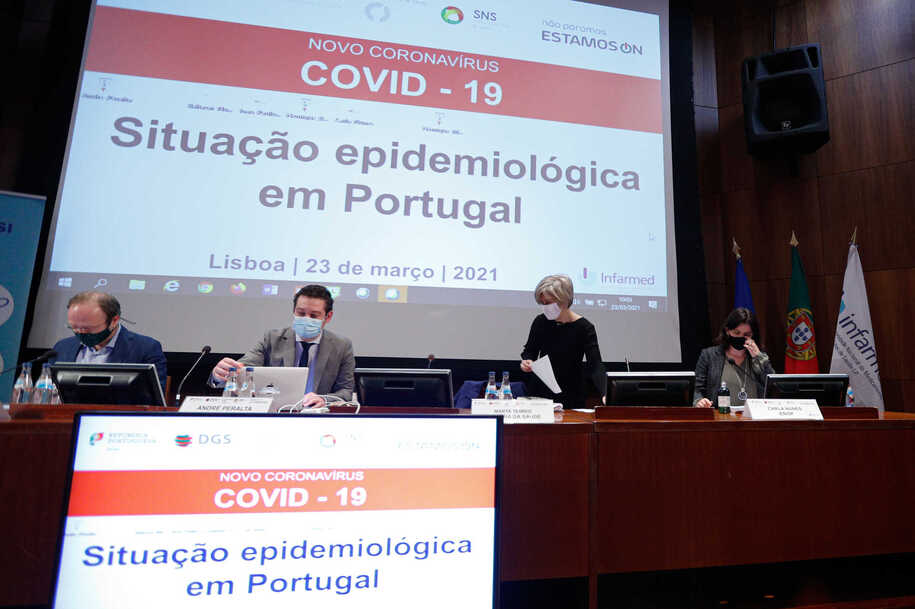
\includegraphics[width=\textwidth]{Imagens/Reunioes_Infarmed.jpg}\\
		\hfill \textcolor{ExecusharesGrey}{\tiny jn.pt, 23 Março 2021. Fonte: Lusa}
	\end{column}
	
	\begin{column}[T]{0.35\textwidth}
		\vspace{0.5cm}
		\textcolor {green}{\Large\textbf{COVID-19 inCTRL}}\\
		\vspace{-0.2cm}
		\textcolor{ExecusharesGrey}{\tiny\hspace{1em}Financiado pelo programa:}\\
		\vspace{-0.2cm}
		\textcolor{ExecusharesGrey}{\tiny\hspace{1em}RESEARCH4COVID - FCT}\\
		\vspace{0.5cm}
		
\includegraphics[width=\textwidth]{Imagens/logo_utad_completo_azul.png}\\
		\vspace{0.3cm}
		
\includegraphics[width=\textwidth]{Imagens/logoentidade_INSA.png}\\
		%Bolsa Refª: COVID_inCTRL/DEP/01/2020\\
		%(de 11 Nov. 2020 até 10 Maio 2021)
	\end{column}
\end{columns}
\end{frame}

%% Modelos Epidemiológicos
\begin{frame}{Modelos Epidemiológicos}
\begin{columns}
	\begin{column}[T]{0.5\textwidth}
	\centering
		\vspace{0.2cm}
		\alert{\large Modelo SIR}\\
		\vspace{0.5cm}
		
\includegraphics[width=\textwidth]{Imagens/SIR_diagram.png}\\
		\vspace{-0.2cm}
		\begin{equation*}
		    \begin{cases}
			    \frac{dS}{dt} = -\beta \frac{S I}{N}\\
			    \frac{dI}{dt} = \frac{S I}{N} - \gamma I\\
			    \frac{dR}{dt} = \gamma I
		    \end{cases}
		\end{equation*}
		
		% Kermack-eta-A.-G.-McKendrick
		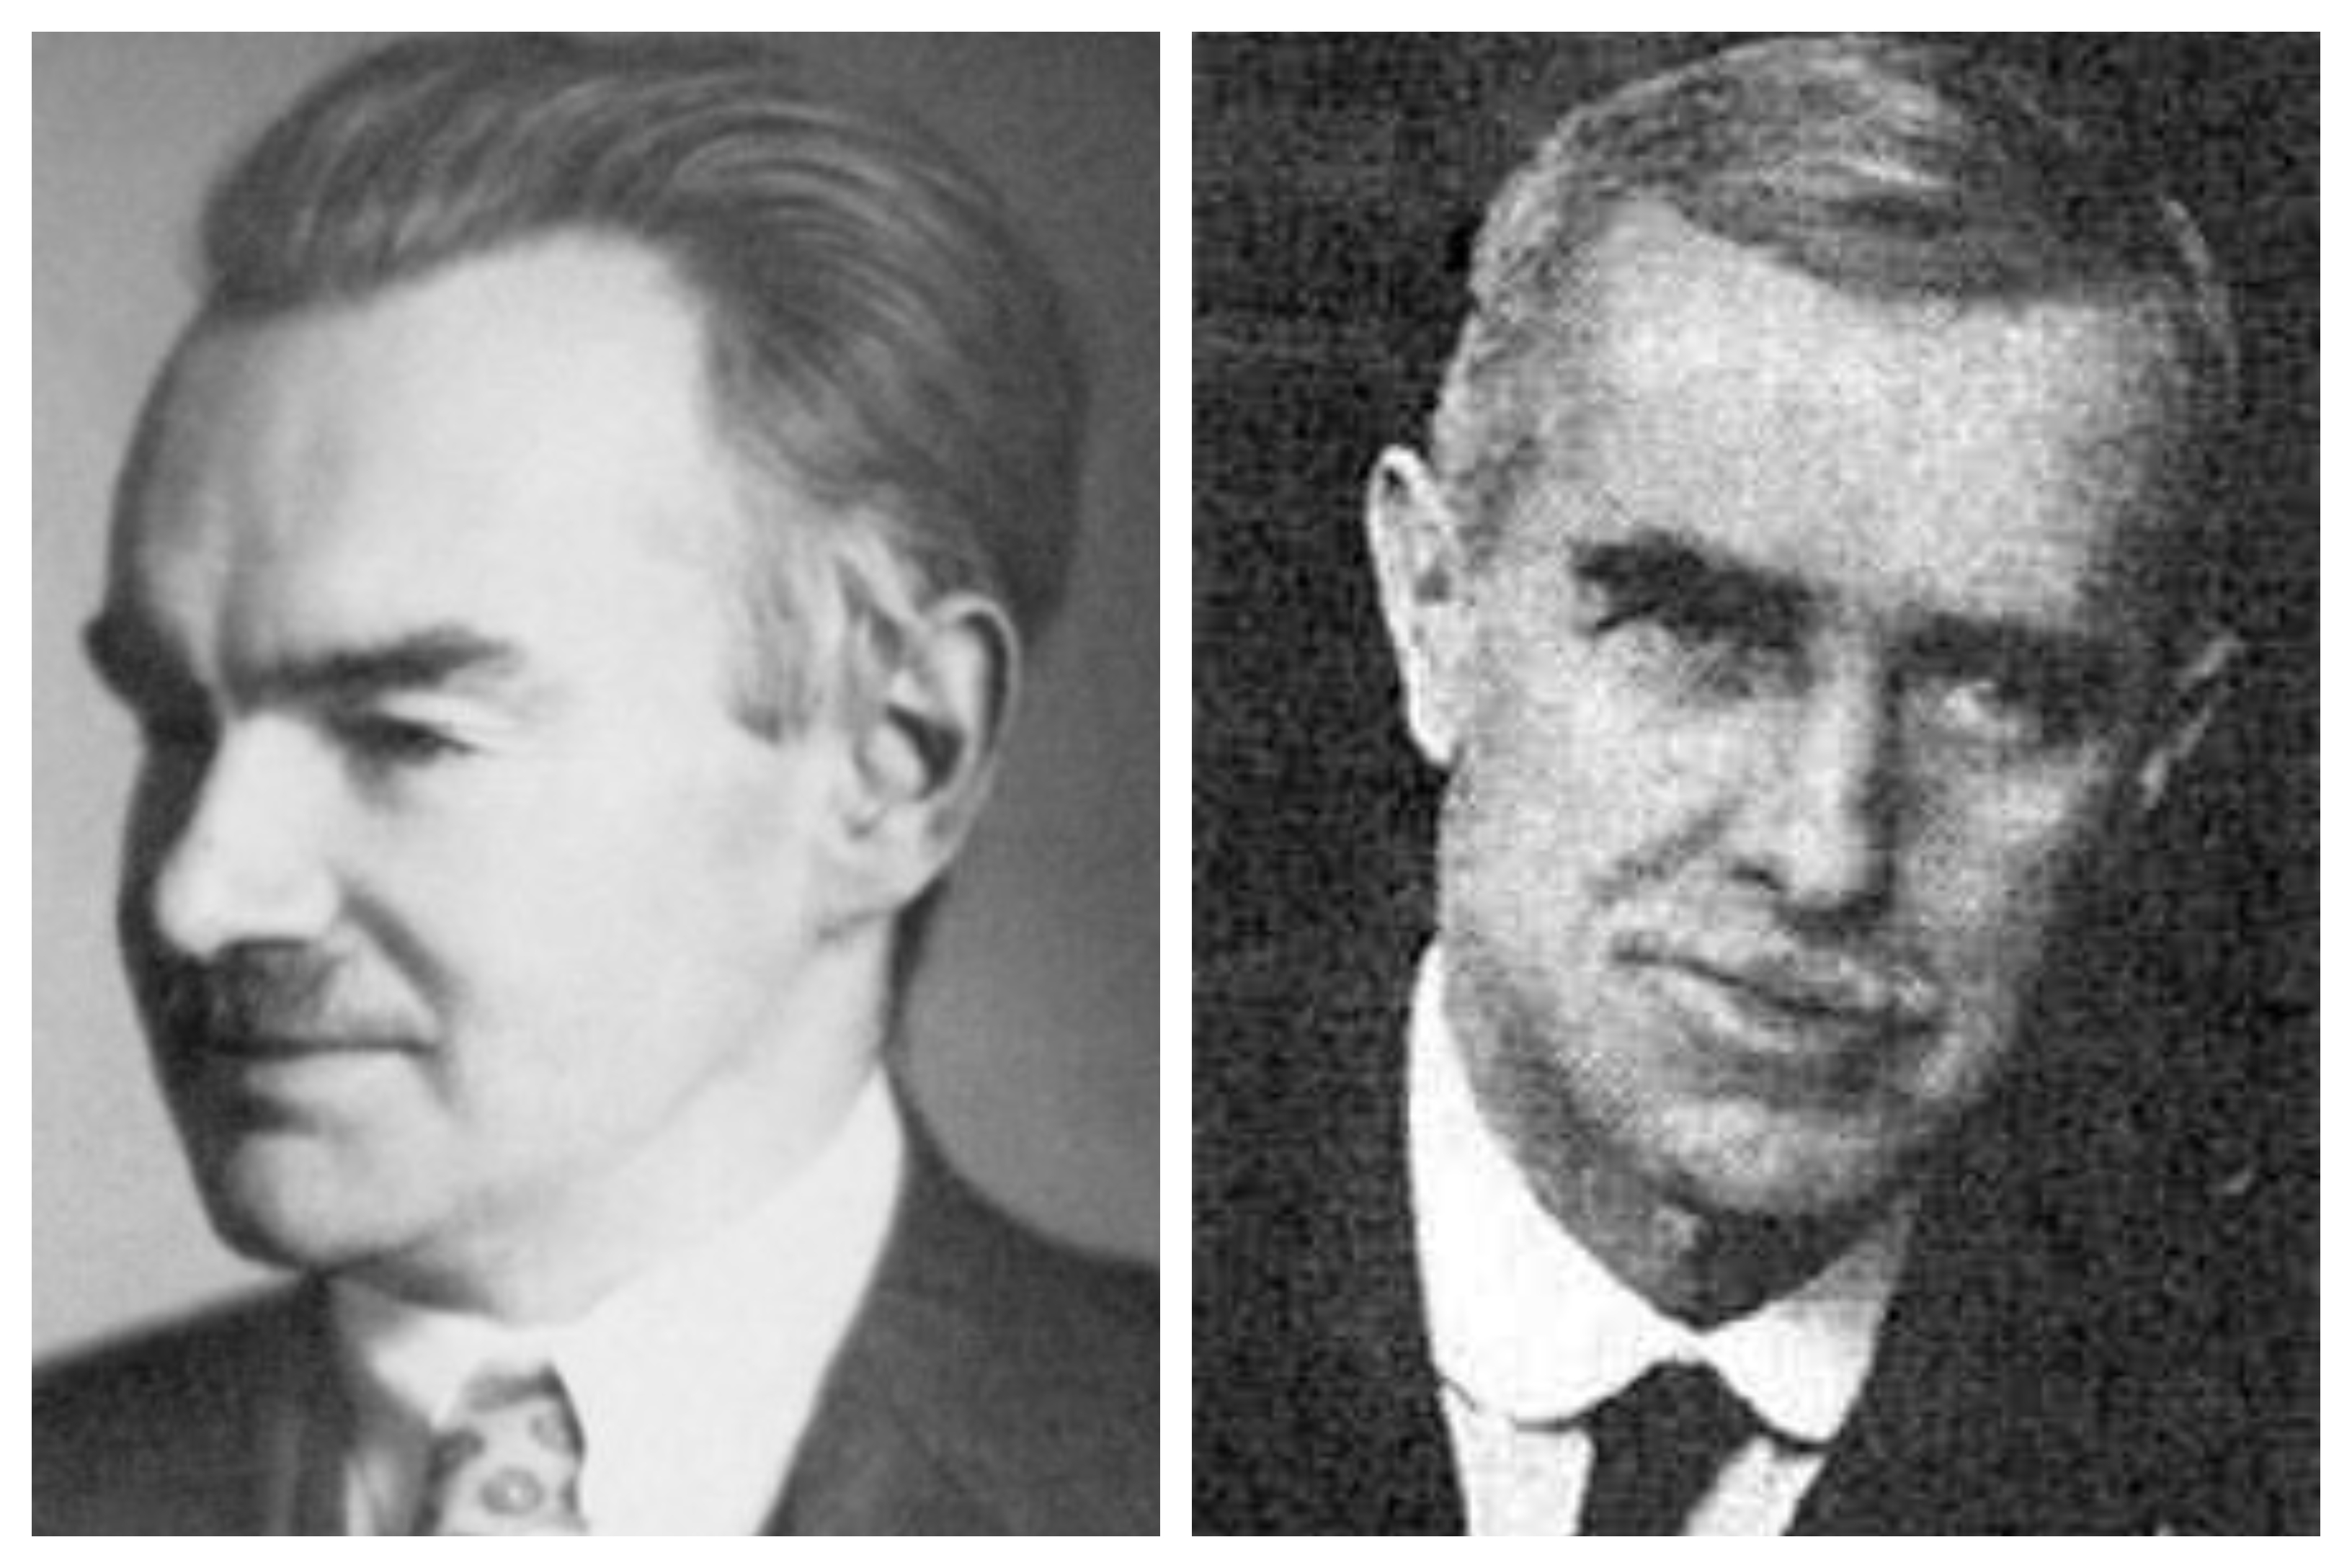
\includegraphics[width=0.5\textwidth]{Imagens/Kermack-eta-A.-G.-McKendrick.jpg}\\
		\textcolor{ExecusharesGrey}{\tiny W.O. Kermack e A.G. McKendrick}\\
	\end{column}
	
	\begin{column}[T]{0.5\textwidth}
		\centering
		\vspace{1.8cm}
		\alert{\large Modelo SEIR}\\
		\vspace{0.5cm}
		
\includegraphics[width=\textwidth]{Imagens/SEIR_diagram.png}\\
		\vspace{-0.2cm}
		\begin{equation*}
		    \begin{cases}
			    \frac{dS}{dt} = -\beta \frac{S I}{N}\\
			    \frac{dE}{dt} = \beta \frac{S I}{N} - \epsilon E\\
			    \frac{dI}{dt} = \epsilon E - \gamma I\\
			    \frac{dR}{dt} = \gamma I
		    \end{cases}
		\end{equation*}
		
	\end{column}
\end{columns}
\end{frame}

%% COVID-19 inCTRL model
\begin{frame}{Modelos Epidemiológicos}
\begin{columns}
	\begin{column}[T]{0.6\textwidth}
		\centering
		\vspace{0.6cm}
		\alert{\large Modelo COVID-19 inCTRL}\\
		\vspace{0.5cm}
		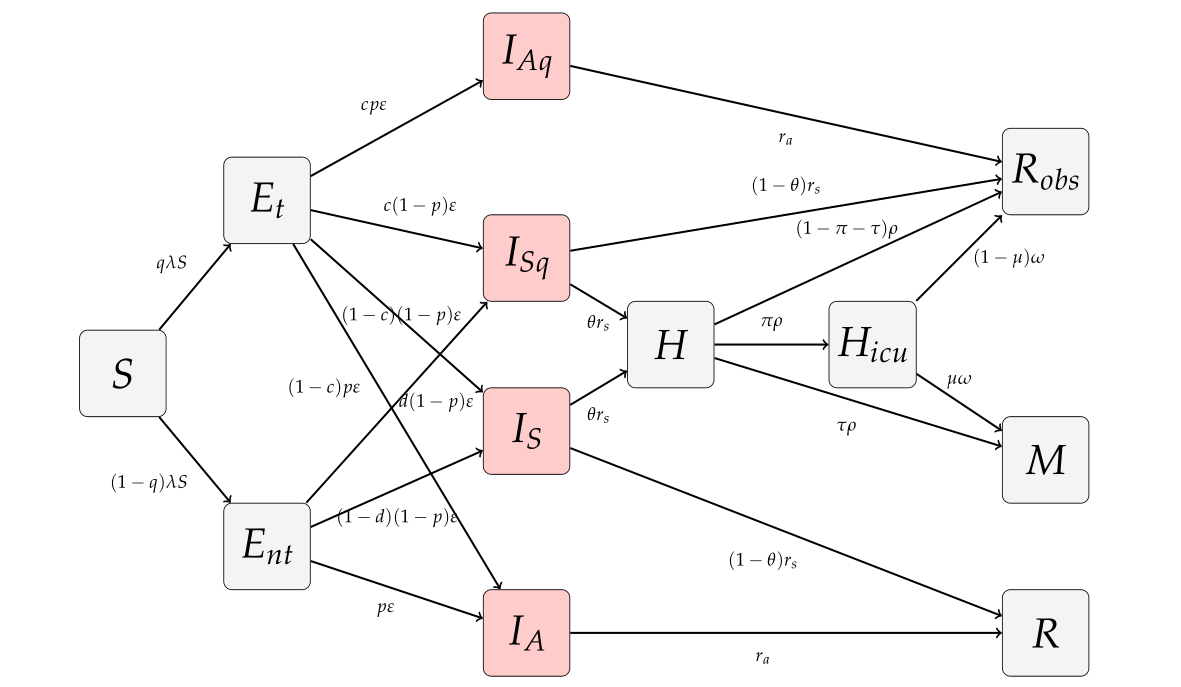
\includegraphics[width=0.8\textwidth]{Imagens/InCTRL_model.png}\\
		\vspace{0.5cm}
		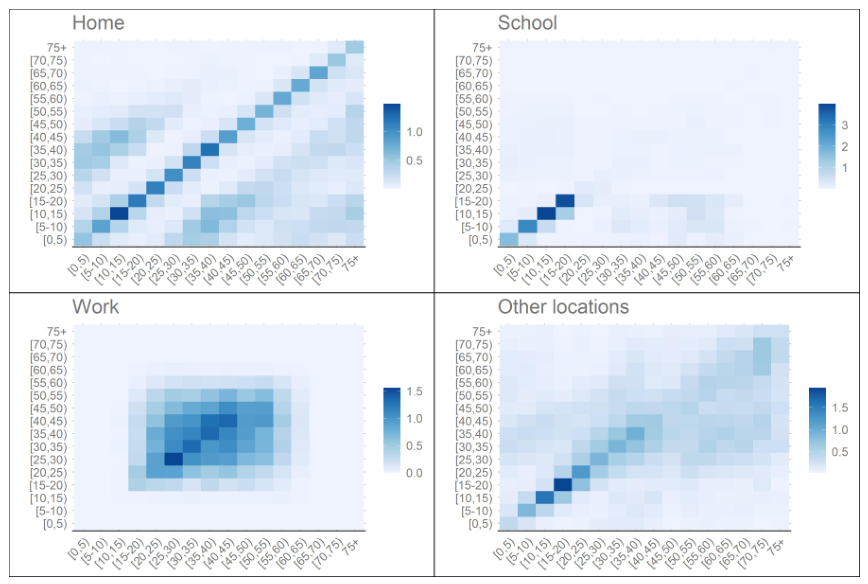
\includegraphics[width=0.7\textwidth]{Imagens/Cont_Matrix.png}\\
	\end{column}
	
	\begin{column}[T]{0.4\textwidth}
		\vspace{0.4cm}
		\scalebox{0.6}{$
		        \begin{aligned}
		            S' &= -\lambda S,\\
		            E'_t &= q \lambda S - \epsilon E_t\\
		            I'_A &= p \epsilon E_{nt} + (1-c)p \epsilon E_t - r_a I_A\\
		            I'_S &= (1-d)(1-p) \epsilon E_{nt} + (1-c)(1-p) \epsilon E_t \\ & -  r_s I_S\\
		            E'_{nt} &= (1-q) \lambda S - \epsilon E_{nt}\\
		            I'_{Aq} &= c p \epsilon E_t - r_a I_{Aq}\\
		            I'_{Sq} &= c(1-p) \epsilon E_t + d (1-p) \epsilon E_{nt} - r_s I_{Sq}\\
		            H' &= \theta r_s (I_S + I_{Sq}) - \rho H\\
		            H'_{icu} &= \pi \rho H - \omega H_{icu}\\
		            M' &= \mu \omega H_{icu} + \tau \rho H\\
		            R'_{obs} &= (1-\theta) r_s I_{Sq} + r_a I_{Aq} + (1-\pi-\tau)\rho H \\ & + (1-\mu)\omega H_{icu}\\
		            R' &= (1-\theta) r_s I_S + r_a I_A
		        \end{aligned}
		$}
		\vspace{0.2cm}
		\vfill
		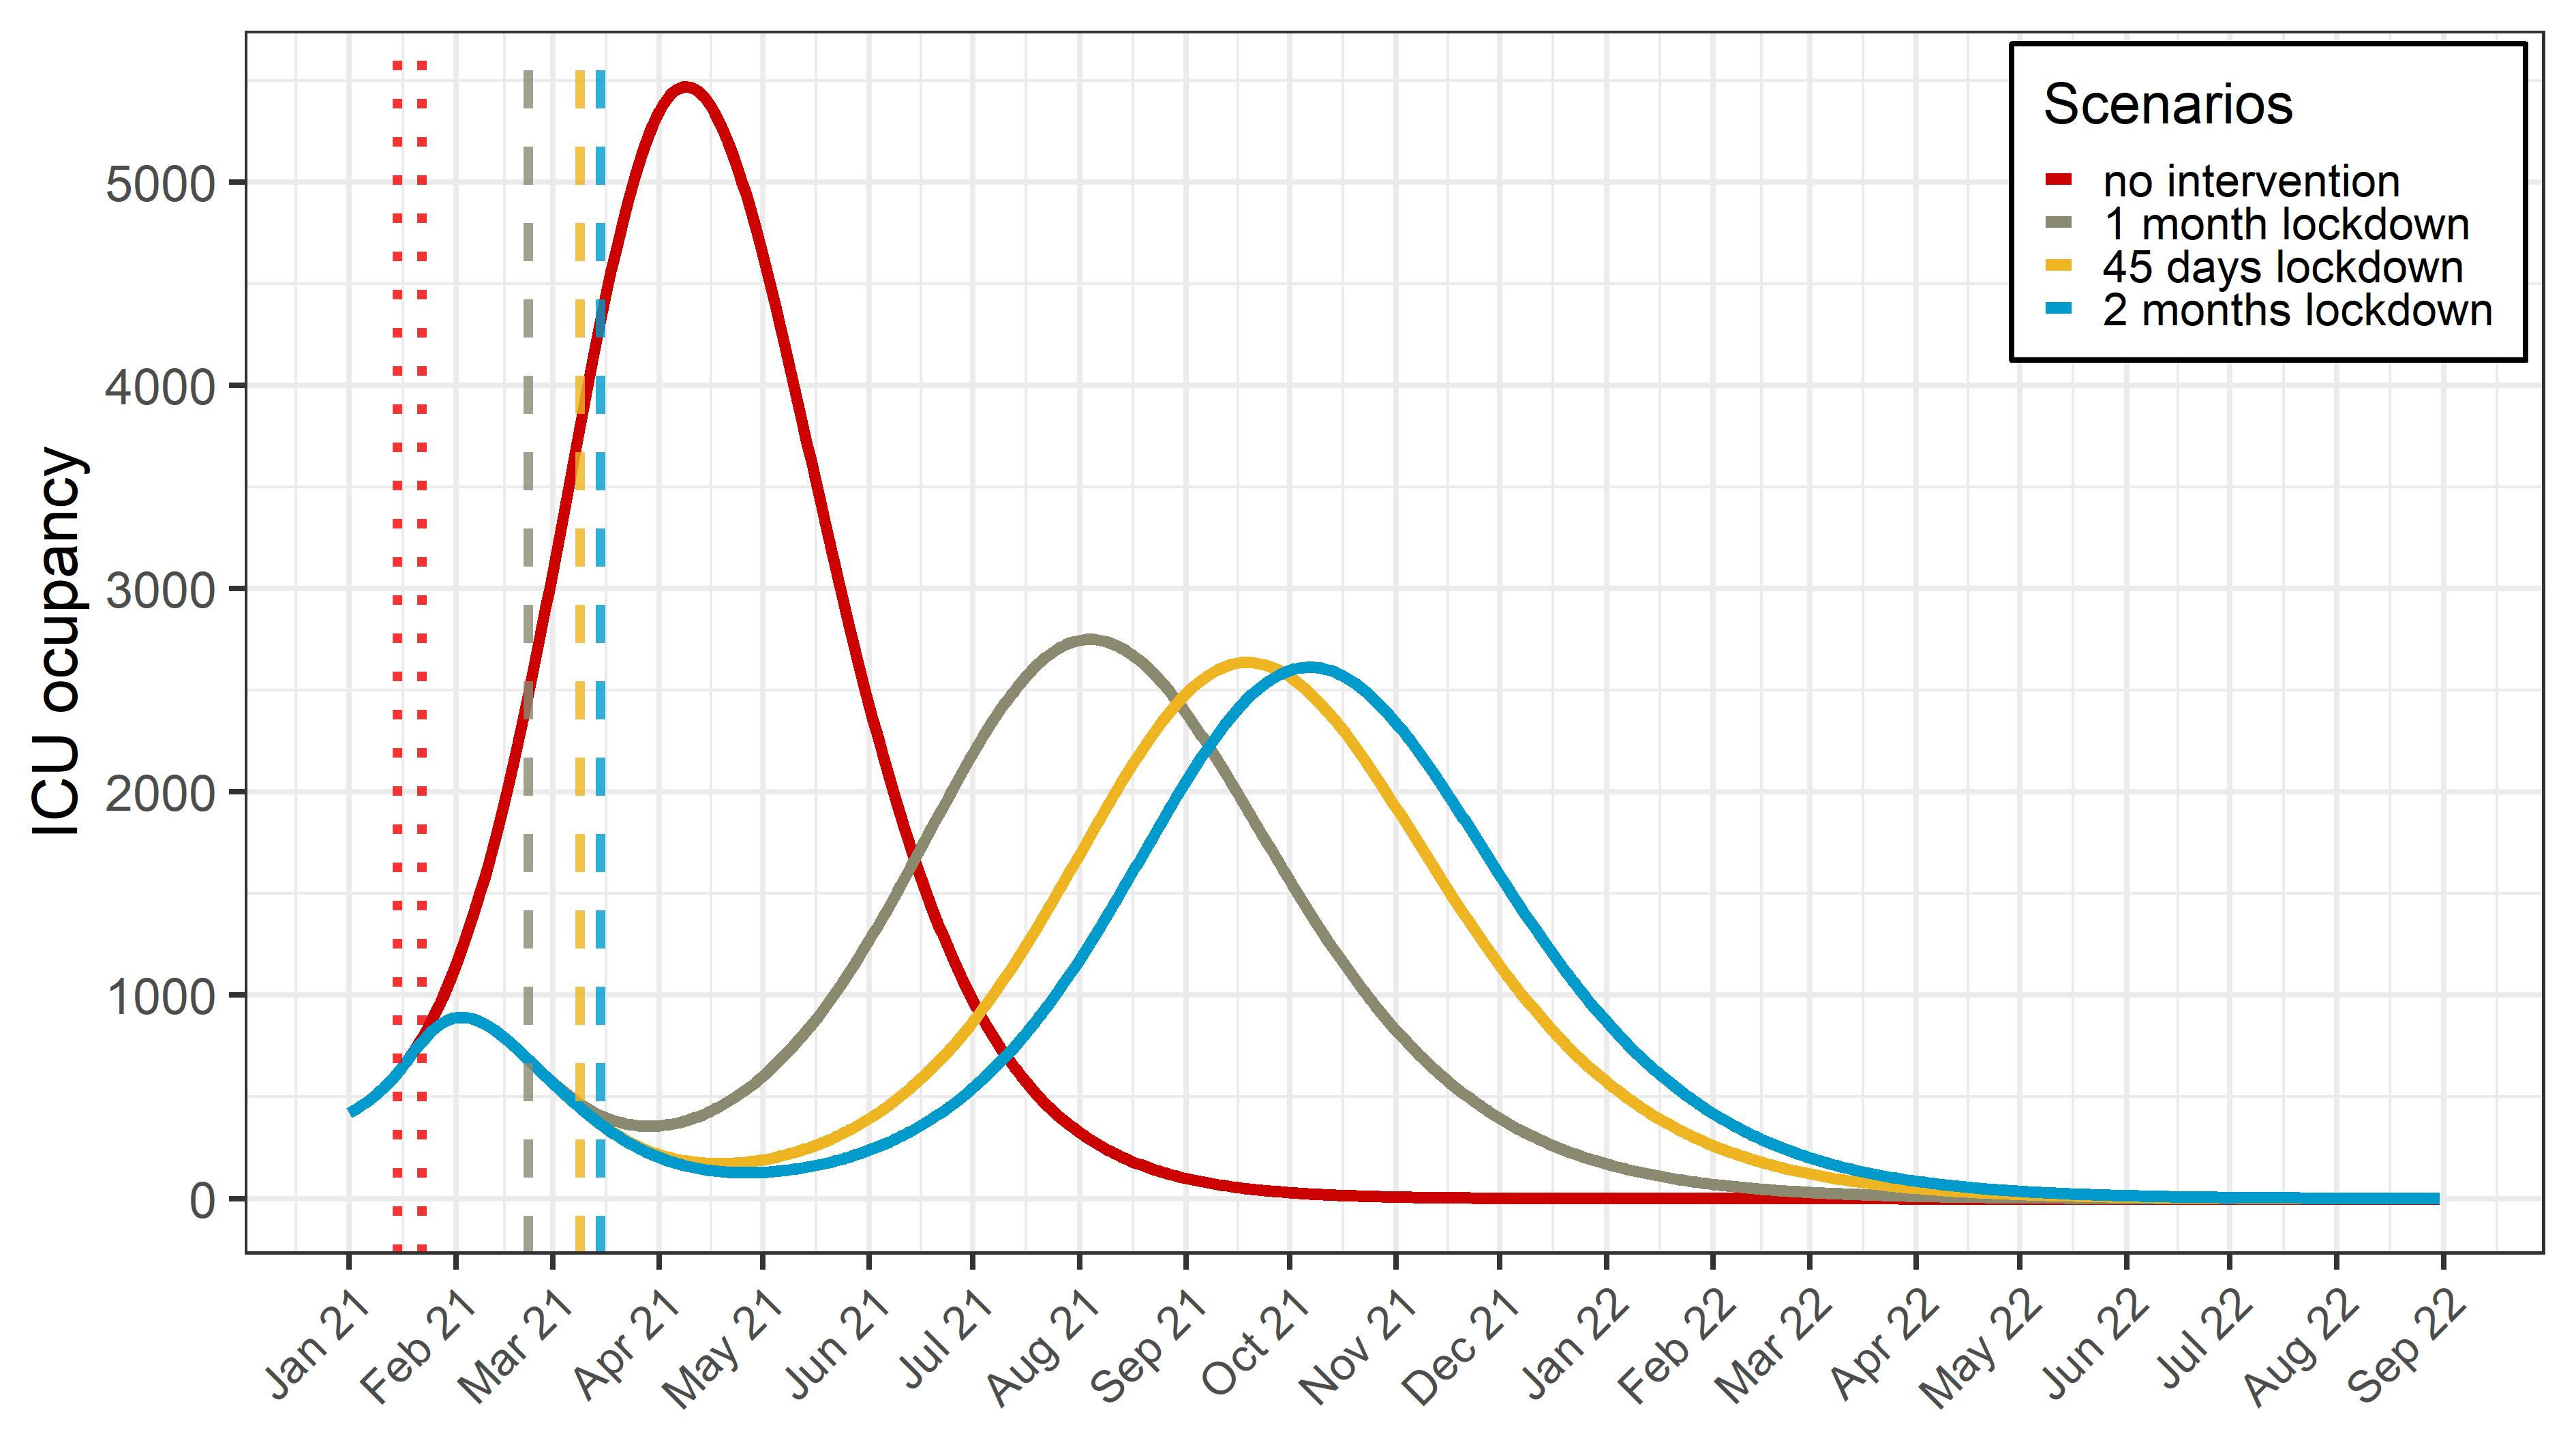
\includegraphics[width=\textwidth]{Imagens/inCTRL_Scenarios_ICU.jpg}\\
	\end{column}
\end{columns}
\end{frame}

%% Análise exploratória
\begin{frame}{Análise exploratória}
\textbf{\Large Como realizar uma Análise exploratória?}
\vspace{0.2cm}
\begin{enumerate}
\item<2-> Obtenção dos dados
\item<3-> Processamento
\item<4-> Transformação
\item<5-> Exploração
\item<6-> Resultados
\end{enumerate}
\end{frame}

%% Obtenção dos dados
\begin{frame}{Obtenção dos dados}
\vspace{0.4cm}
\begin{itemize}
\item Os dados são relativos a APR-DRG (all-patient refined diagnosis-related groups) de Portugal, relativamente a pacientes com diagnostico de COVID-19
\item Disponibilizados pelos SPMS /ACSS de Portugal, na plataforma de acesso restrito BI-MH
\item Entradas de 4 de janeiro 2020 até saídas a 22 de junho de 2021
\item 56 666 entradas/saídas hospitalares registadas (linhas), cada uma contendo 13 variáveis (colunas)
\end{itemize}
\vspace{0.4cm}
Apesar da informação contida ser pseudo-anonimizada, por se tratarem de dados hospitalares, \alert{foi necessário a aprovação por um comité ético} a utilização dos dados.
\end{frame}

%% Processamento
\begin{frame}{Processamento}
\vspace{1cm}
\textbf{Objetivo:} Transformar os dados originais para outros mais utilizáveis e verificar possíveis incongruências.
 \begin{enumerate}
\item Identificação das variáveis
\item Alteração de designações
\item Transformação de variáveis  \\ \vspace{-0.2cm} \textcolor{ExecusharesGrey}{\scriptsize \hspace{1em}(ex: idade, grupos etários, LoS, etc.)}
\item Problema de representação \\ \vspace{-0.2cm} \textcolor{ExecusharesGrey}{\scriptsize \hspace{1em}(consideradas apenas entradas entre 1 de Março de 2020 e 31 de Março de 2021)}
\item Remoção de variáveis sem interesse
\end{enumerate}
\vspace{-0.2cm}
\begin{figure}[!ht]
    \centering
    \begin{subfigure}{0.40\textwidth}
	\caption*{Dados Originais}
	\vspace{-0.4cm}
        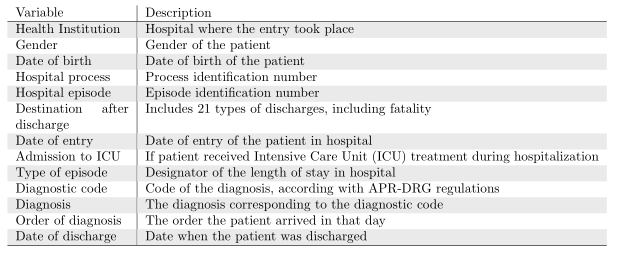
\includegraphics[width=\textwidth, valign=m]{Imagens/Dados_Originais.png}
    \end{subfigure}
\qquad\tikz[baseline=-0.8\baselineskip]\draw[ultra thick,->] (0,0) -- ++ (0.5,0);\qquad
    \begin{subfigure}{0.38\textwidth}
    \caption*{Dados Processados}
    \vspace{-0.4cm}
    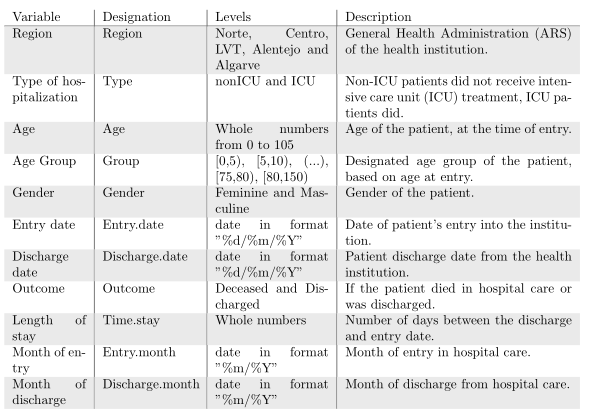
\includegraphics[width=\textwidth, valign=m]{Imagens/Dados_Processados.png}
\end{subfigure}
\end{figure}
\end{frame}

%%Transformação
\begin{frame}{Transformação}
\vspace{0.8cm}
\textbf{Objetivo:} Transformar os dados noutros com nova informação.

\begin{figure}[!ht]
    \centering
    \begin{subfigure}{0.40\textwidth}
	\caption*{Dados Processados}
	\vspace{-0.4cm}
        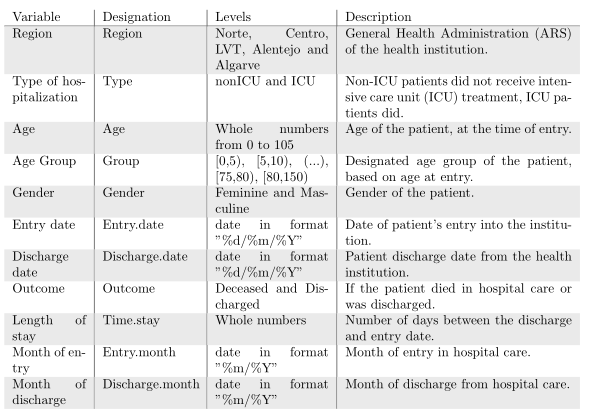
\includegraphics[width=\textwidth]{Imagens/Dados_Processados.png}
    \end{subfigure}
\qquad\tikz[baseline=-2cm]\draw[ultra thick,->] (0,0) -- ++ (0.5,0);\qquad
    \begin{subfigure}{0.38\textwidth}
    \centering
    \caption*{Tempo de permanência}
    \vspace{-0.4cm}
    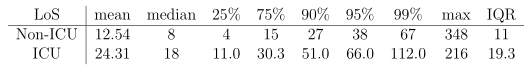
\includegraphics[width=\textwidth]{Imagens/Dados_Transf_Stats.png}\\
    \vspace{0.2cm}
    \caption*{Dados por dia}
    \vspace{-0.4cm}
    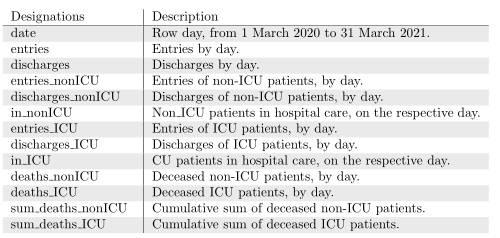
\includegraphics[width=\textwidth]{Imagens/Dados_Transf_byDay.png}\\
    \vspace{0.2cm}
    \caption*{Parâmetros em relação a variáveis}
    \vspace{-0.4cm}
    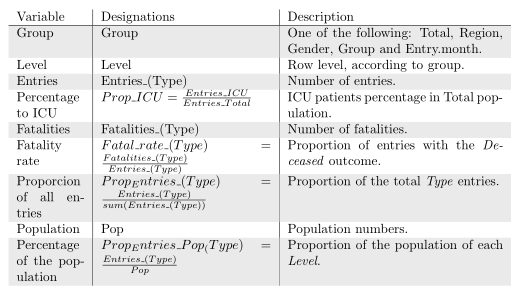
\includegraphics[width=\textwidth]{Imagens/Dados_Transf_Perc.png}\\
\end{subfigure}
\end{figure}

\end{frame}

%% Exploração
\begin{frame}{Exploração}
\textbf{Objetivo:} Relacionar as diferentes variáveis de forma a encontrar relações de interesse, utilizando variados tipos de visualização.

\vspace{2cm}

\begin{figure}
	\centering
	\begin{subfigure}[][40pt][b]{0.3\textwidth}
		\caption*{Diagramas de caixa / Gráficos de violino}
		\vspace{-0.4cm}
    		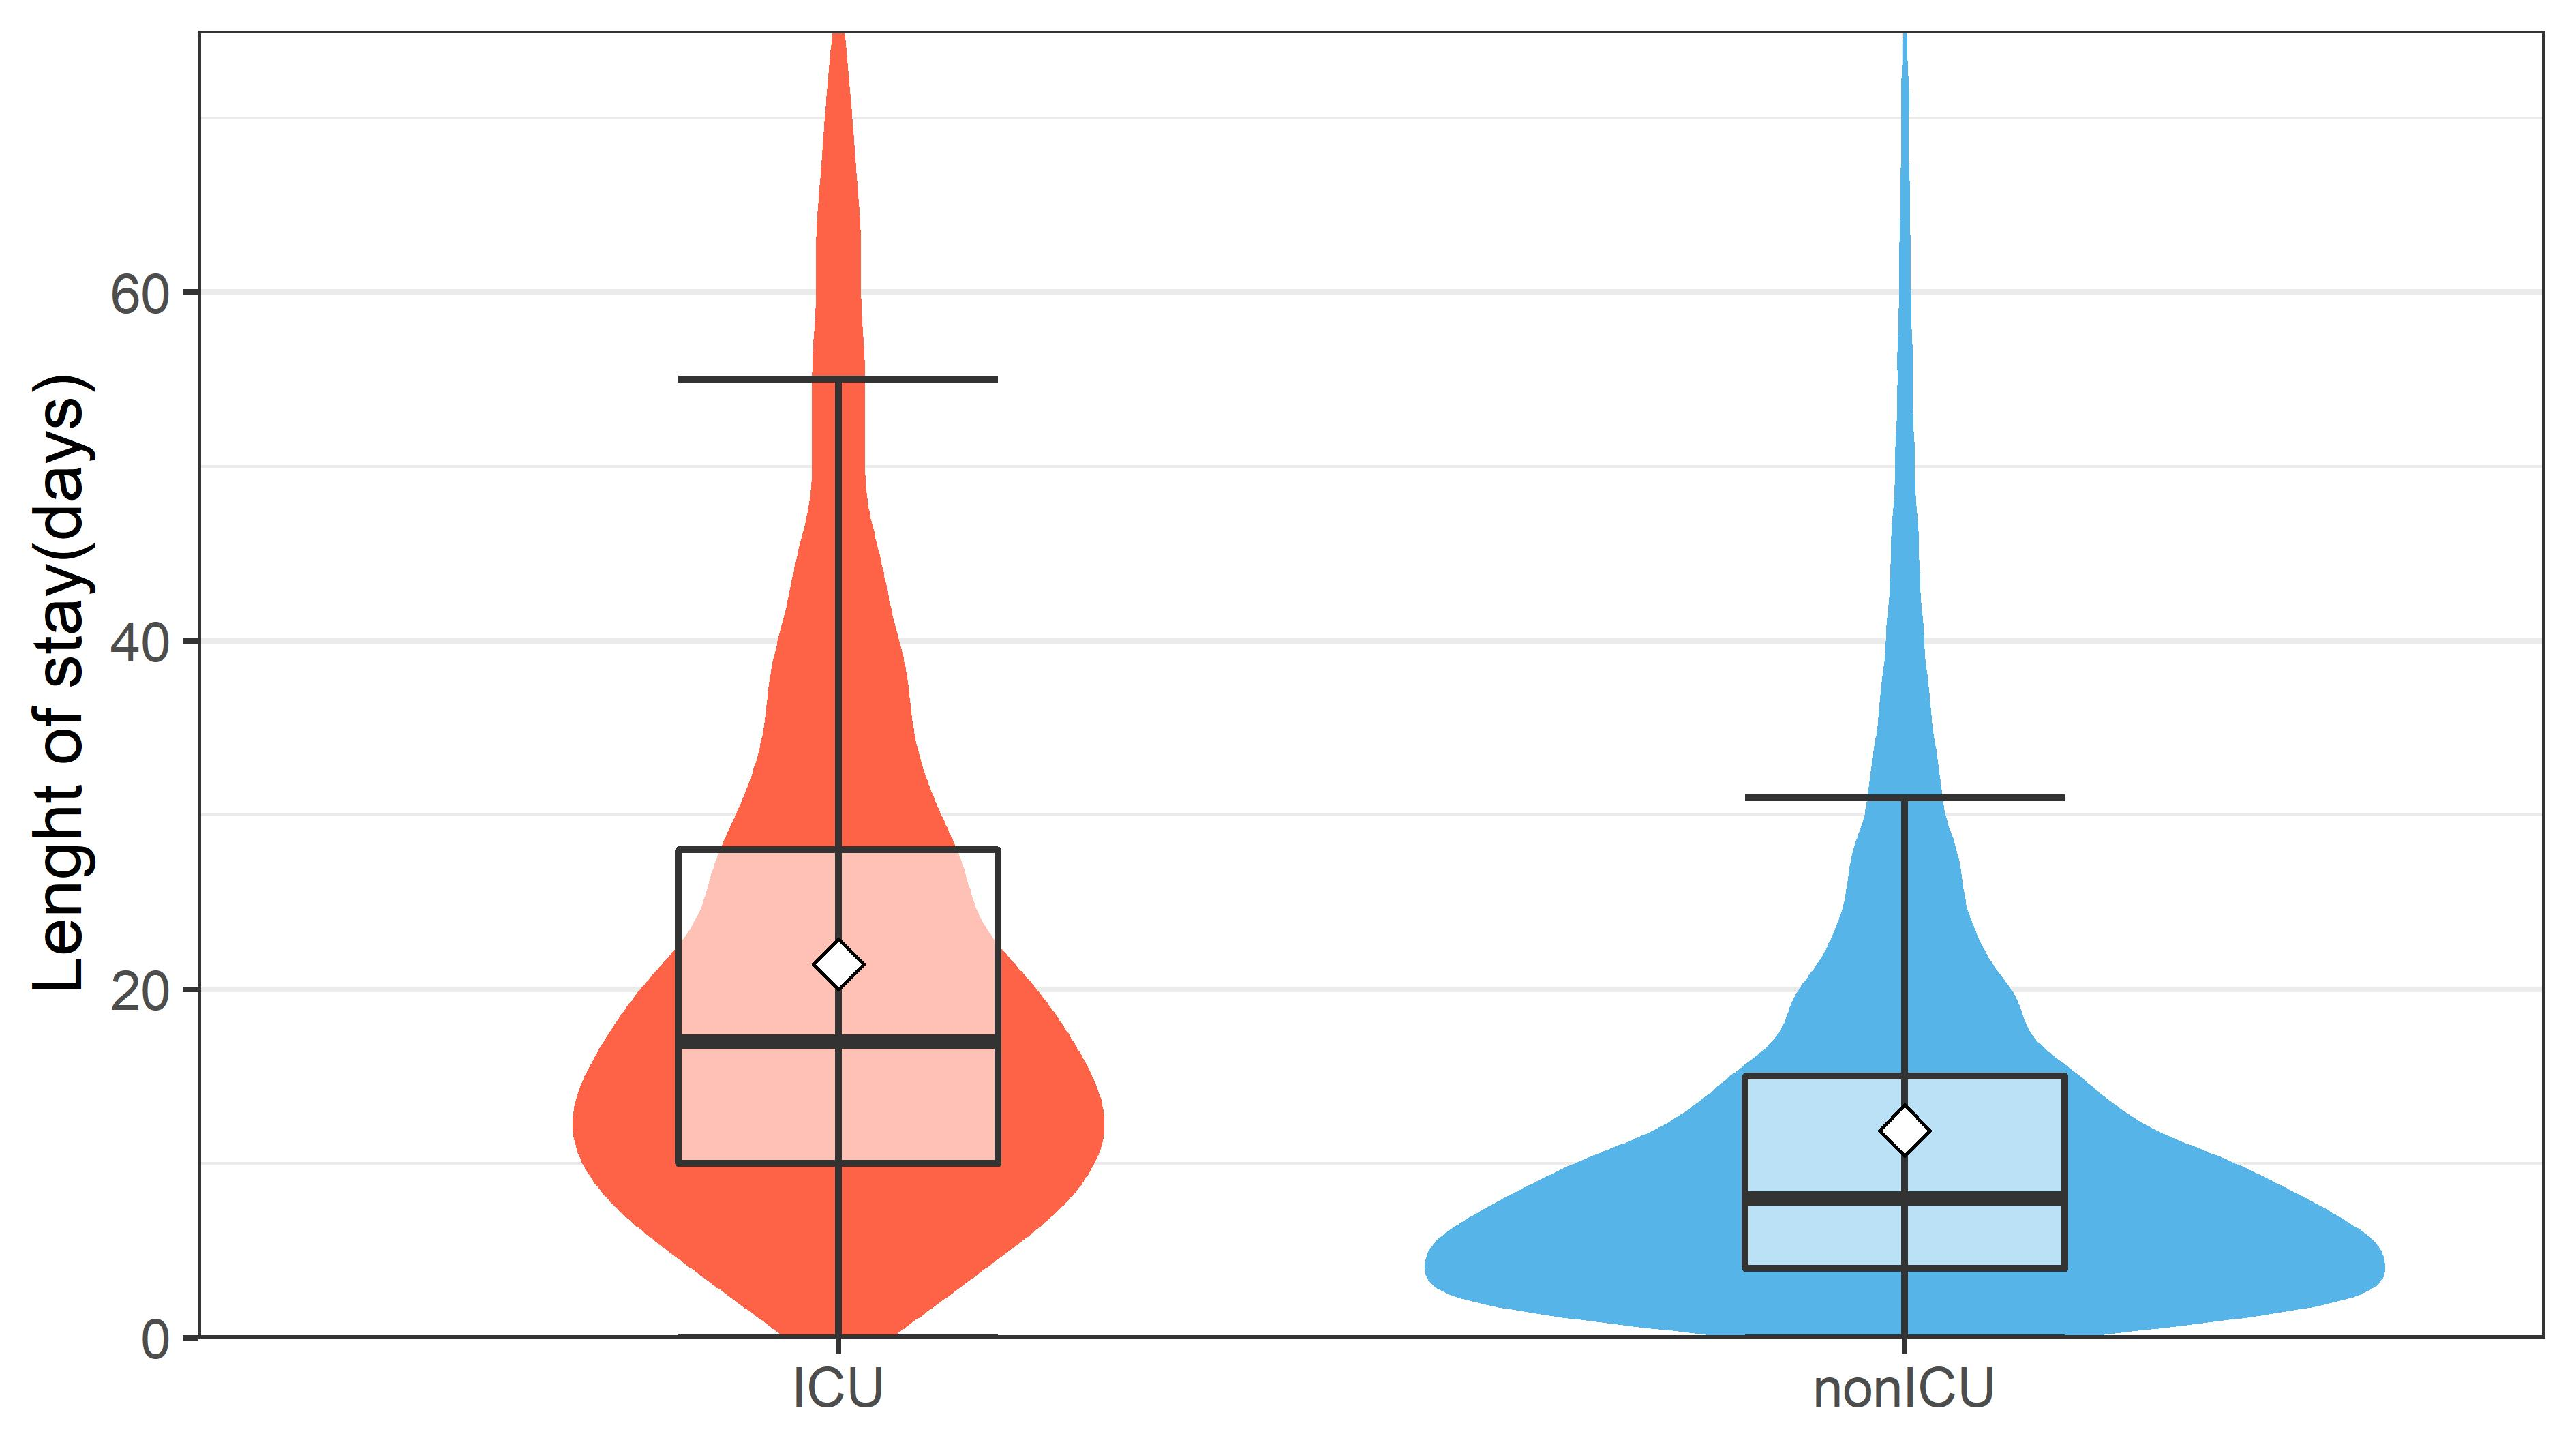
\includegraphics[width=\textwidth]{Imagens/violinBox_Type.jpeg}\\
	\end{subfigure}
	\begin{subfigure}[][40pt][c]{0.3\textwidth}
		\caption*{Gráficos de linha}
		\vspace{-0.4cm}
   		 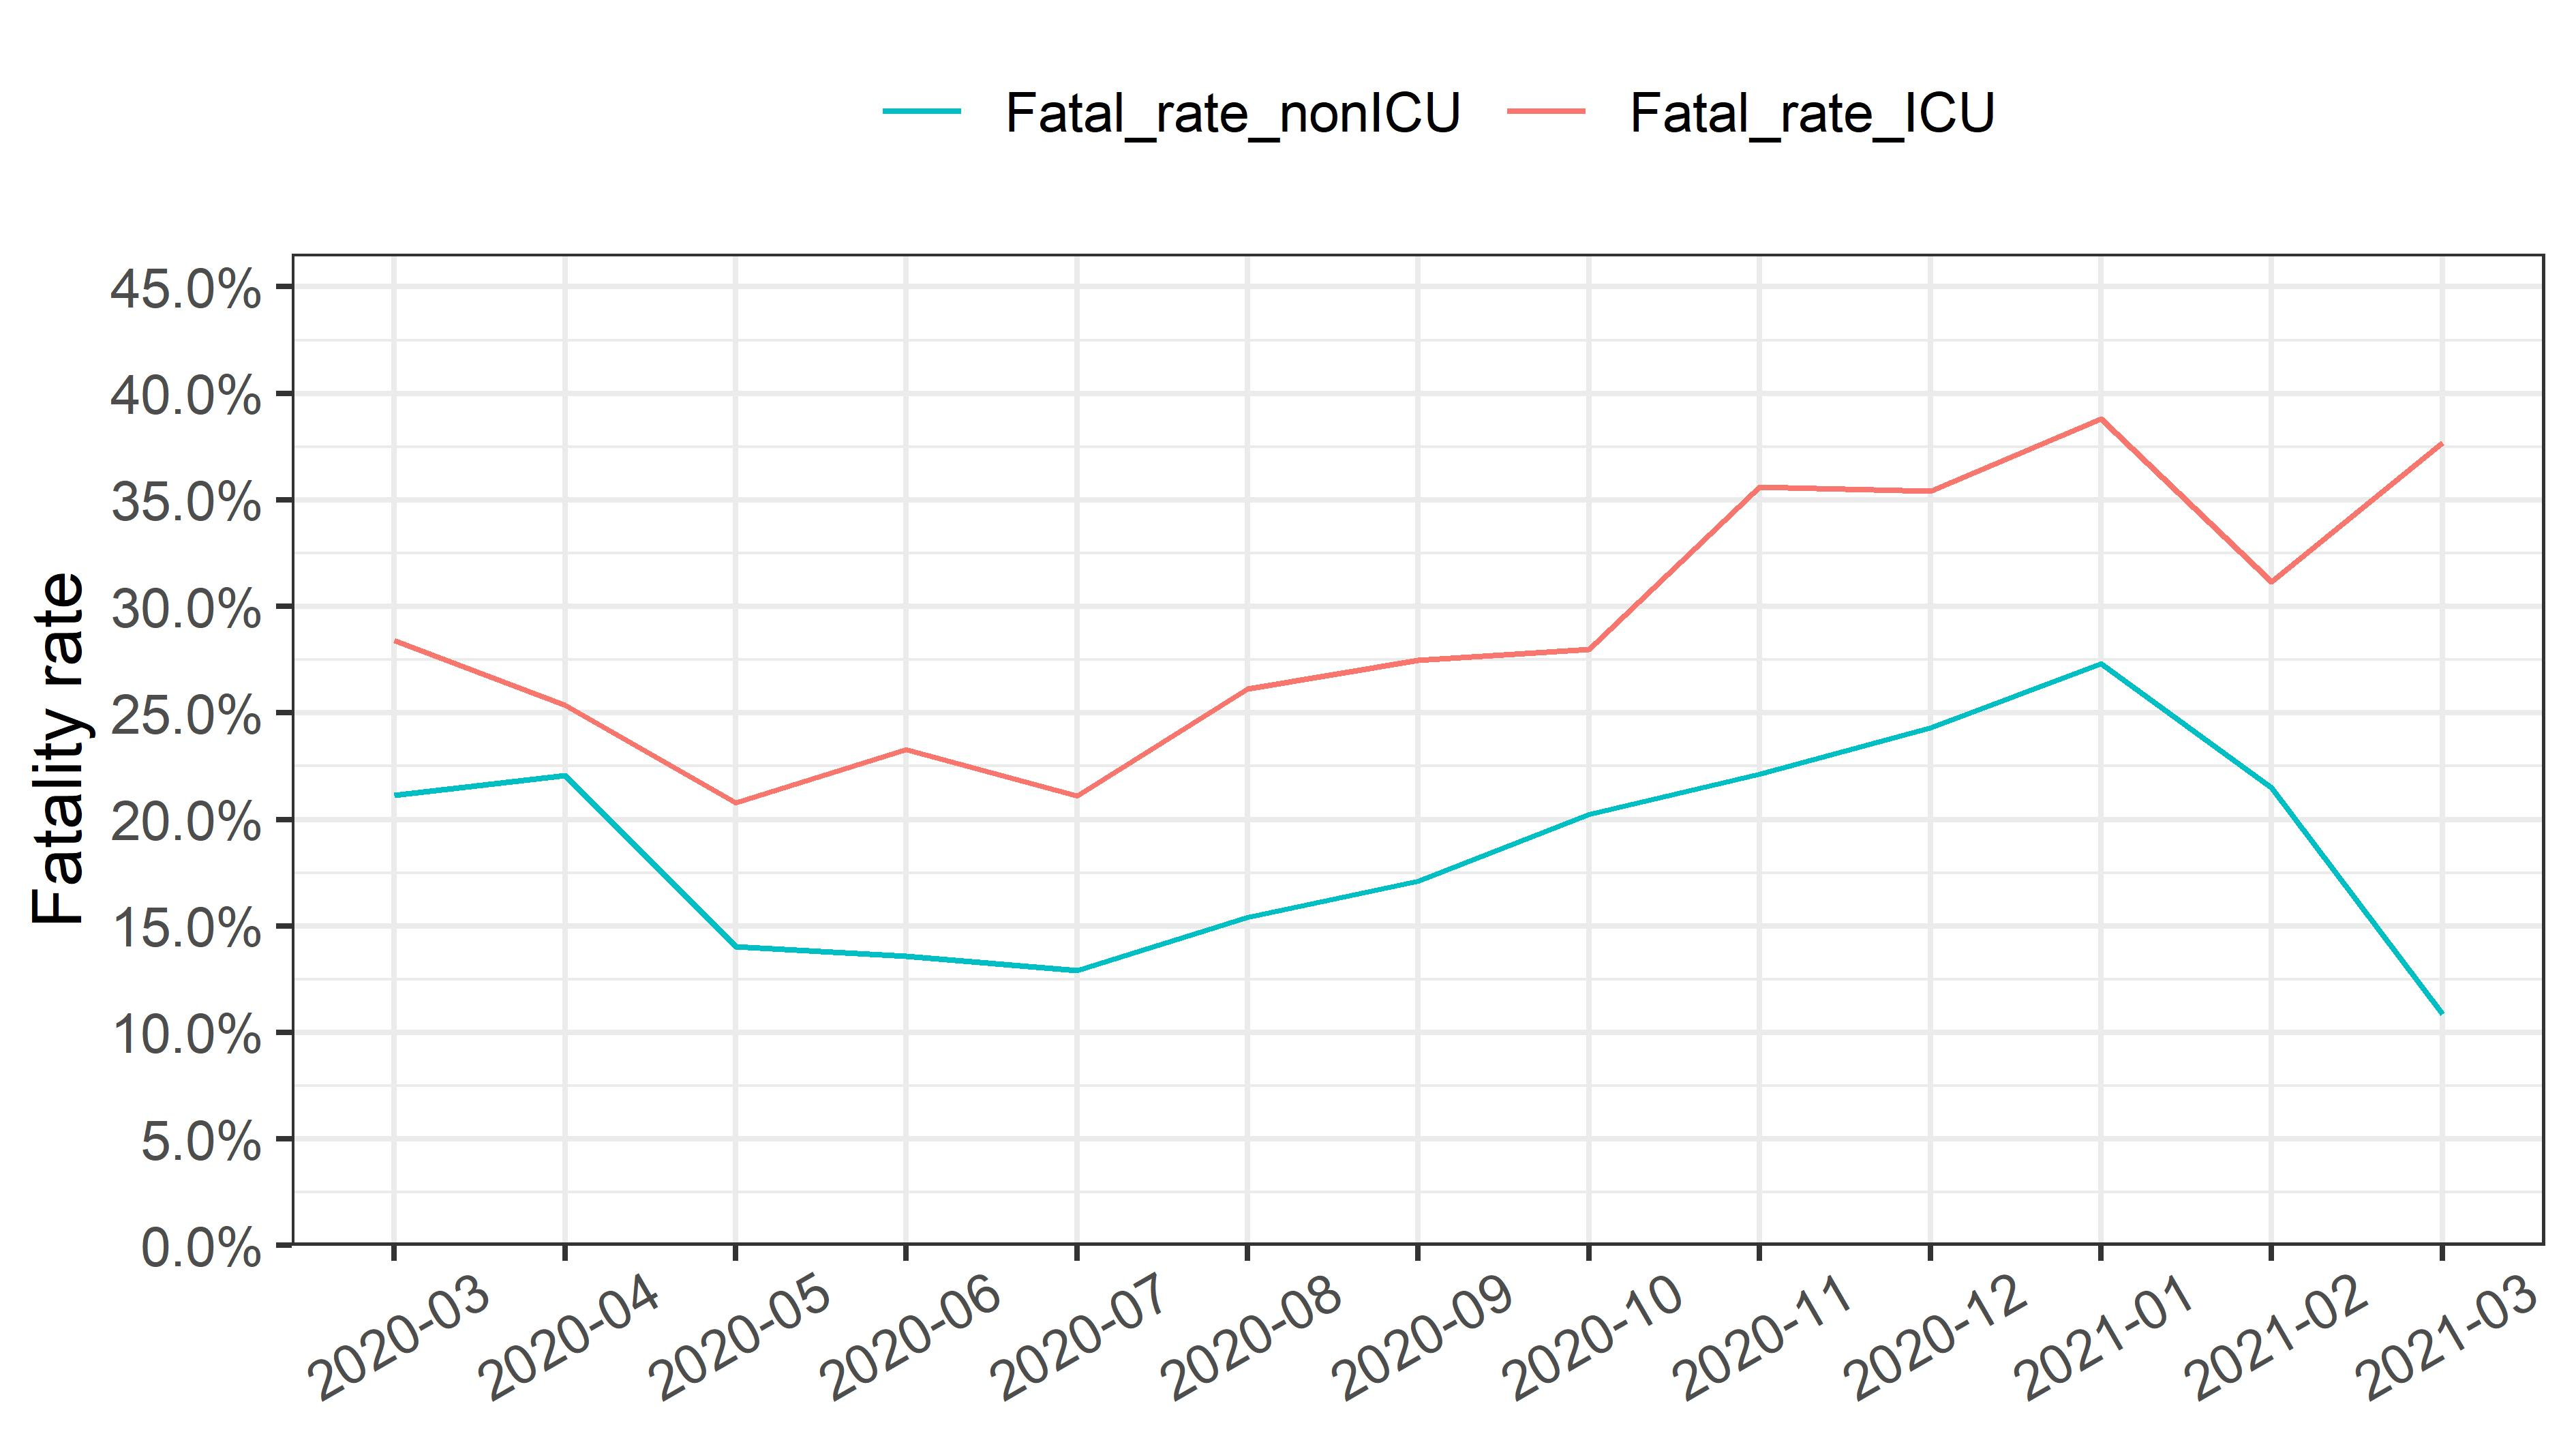
\includegraphics[width=\textwidth]{Imagens/PopVarPlot_fatalRate.jpeg}\\
	\end{subfigure}
	\begin{subfigure}[][40pt][t]{0.3\textwidth}
		\caption*{Gráficos de barras}
		\vspace{-0.4cm}
   		 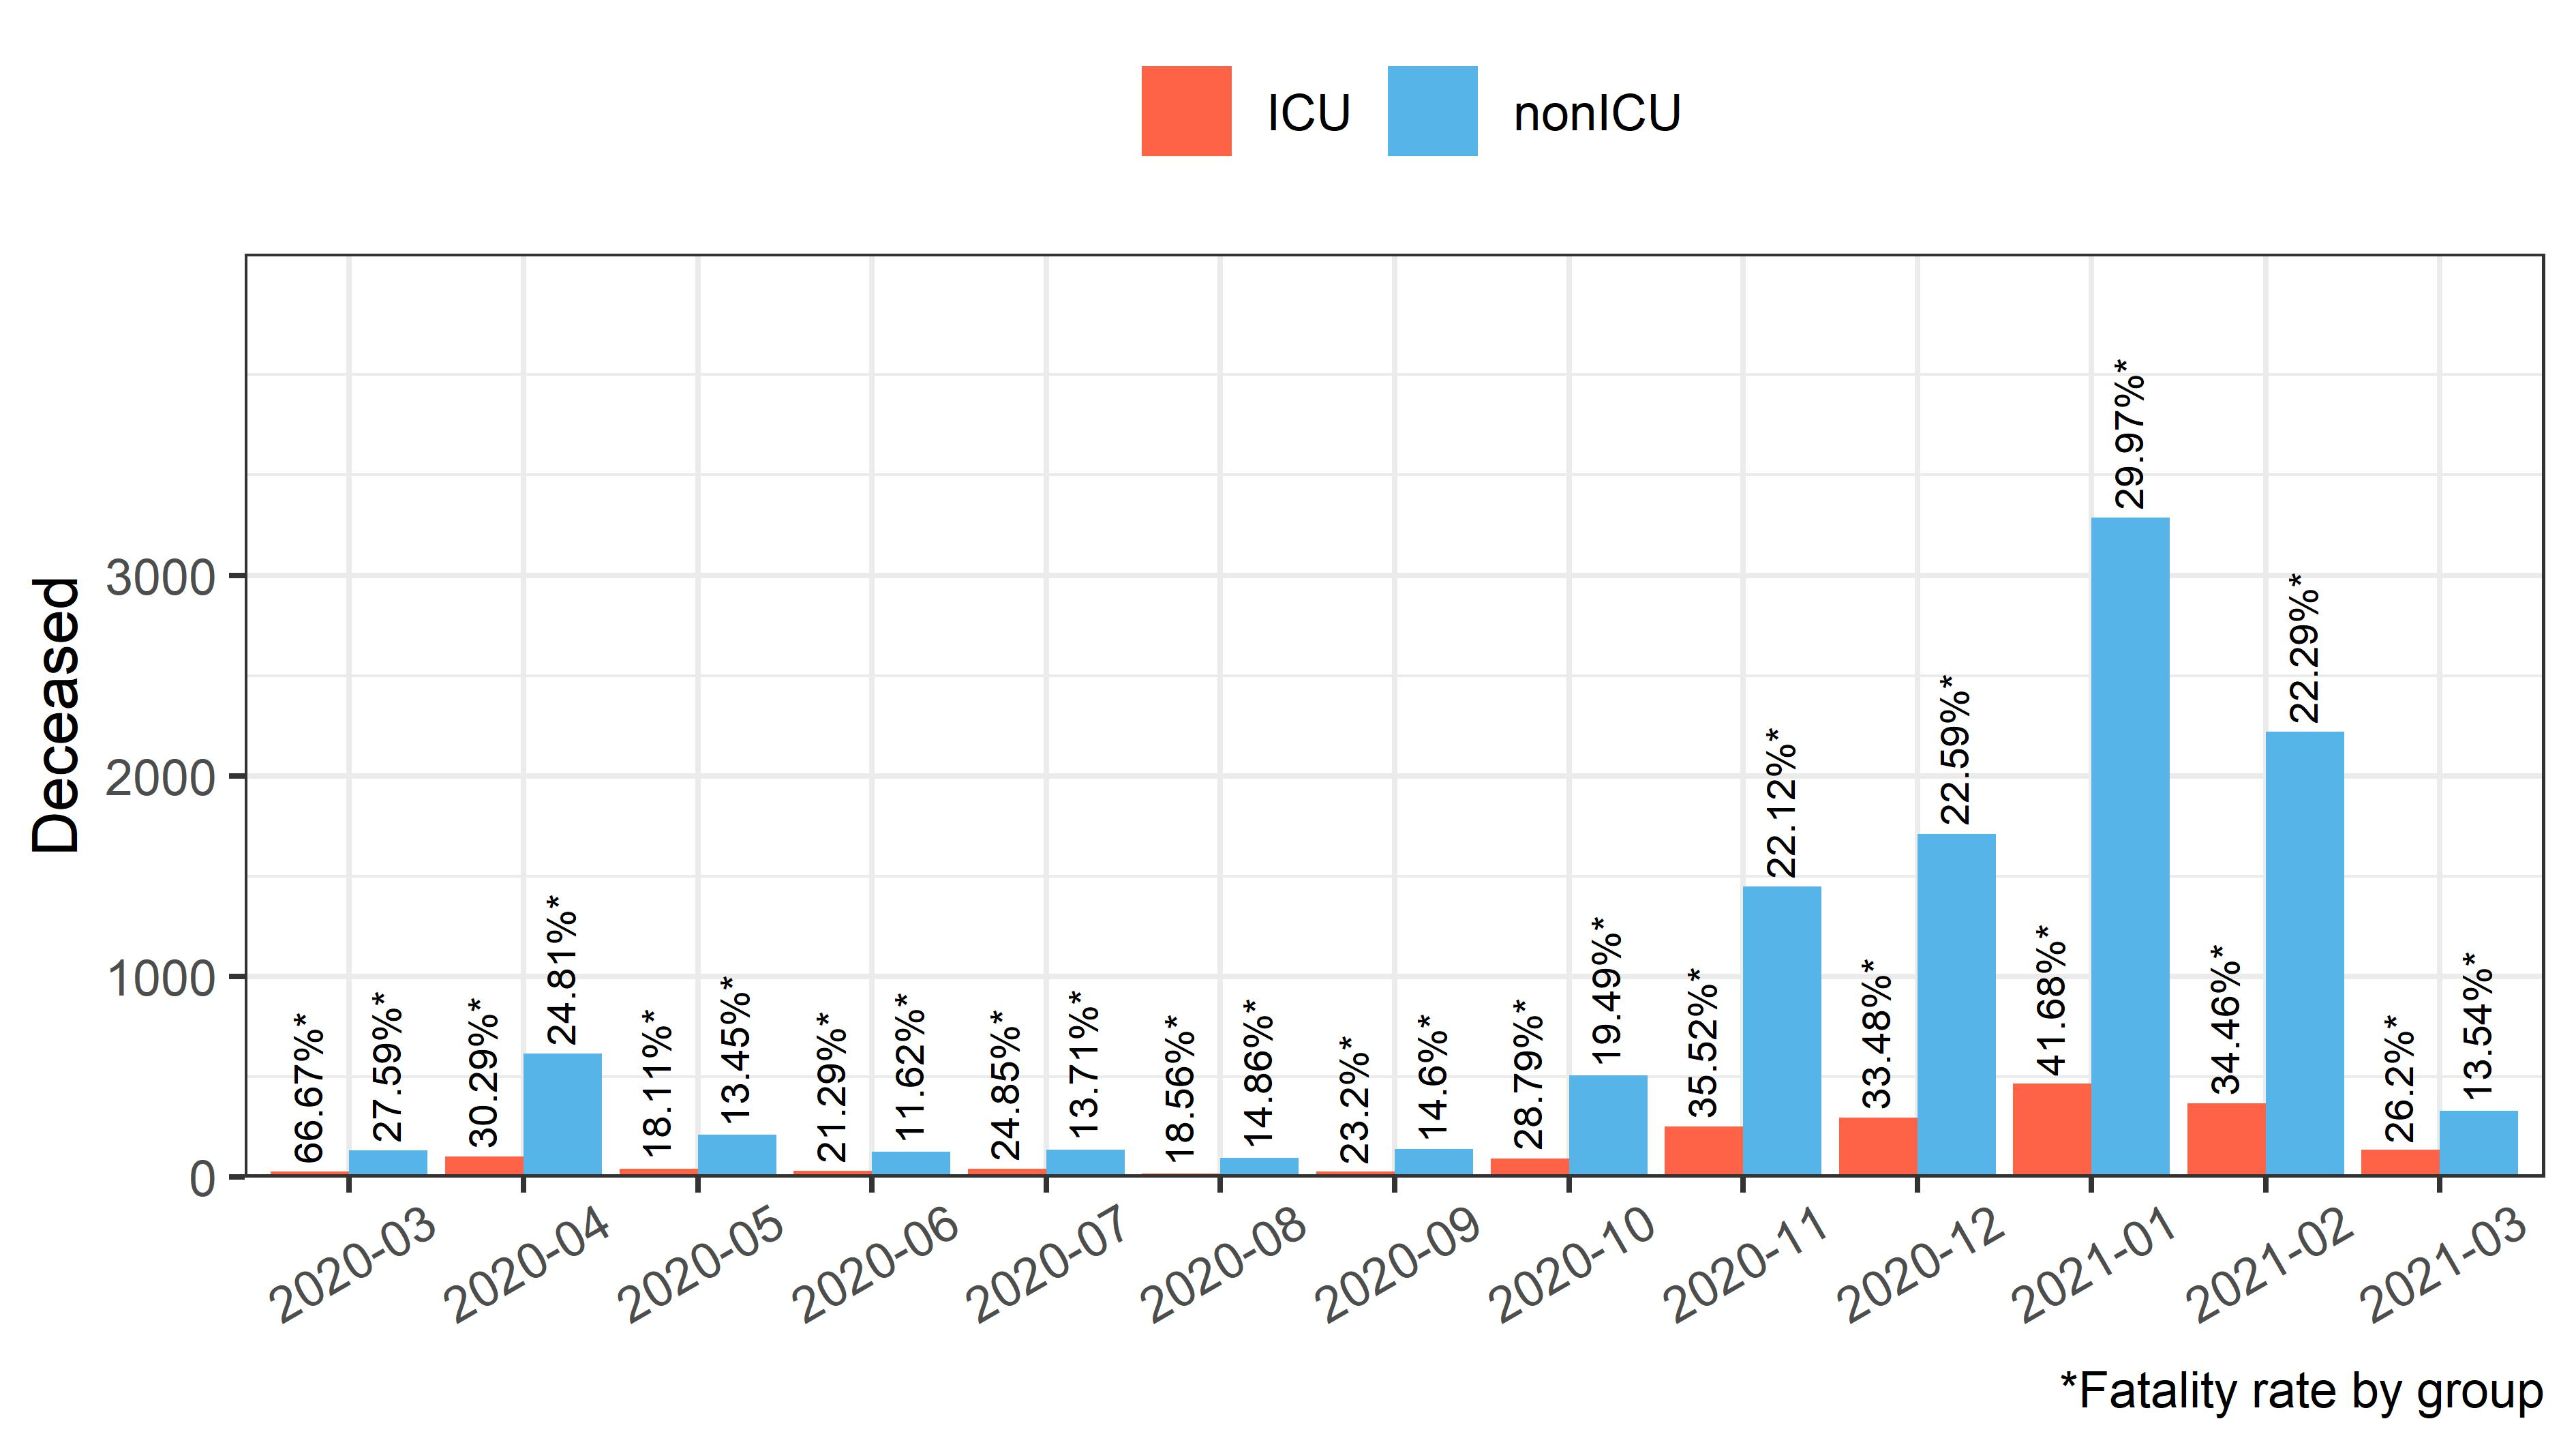
\includegraphics[width=\textwidth]{Imagens/histPlot_Discharge_month_Type_Death.jpeg}\\
	\end{subfigure}
\end{figure}
\end{frame}

%% Exploração
\begin{frame}{Exploração}
\vspace{0.4cm}
\alert{\large Variáveis a comparar}
\begin{figure}
\centering
\begin{subfigure}{0.3\textwidth}
\caption*{Tipo de hospitalização (com e sem UCI)}
\vspace{-0.4cm}
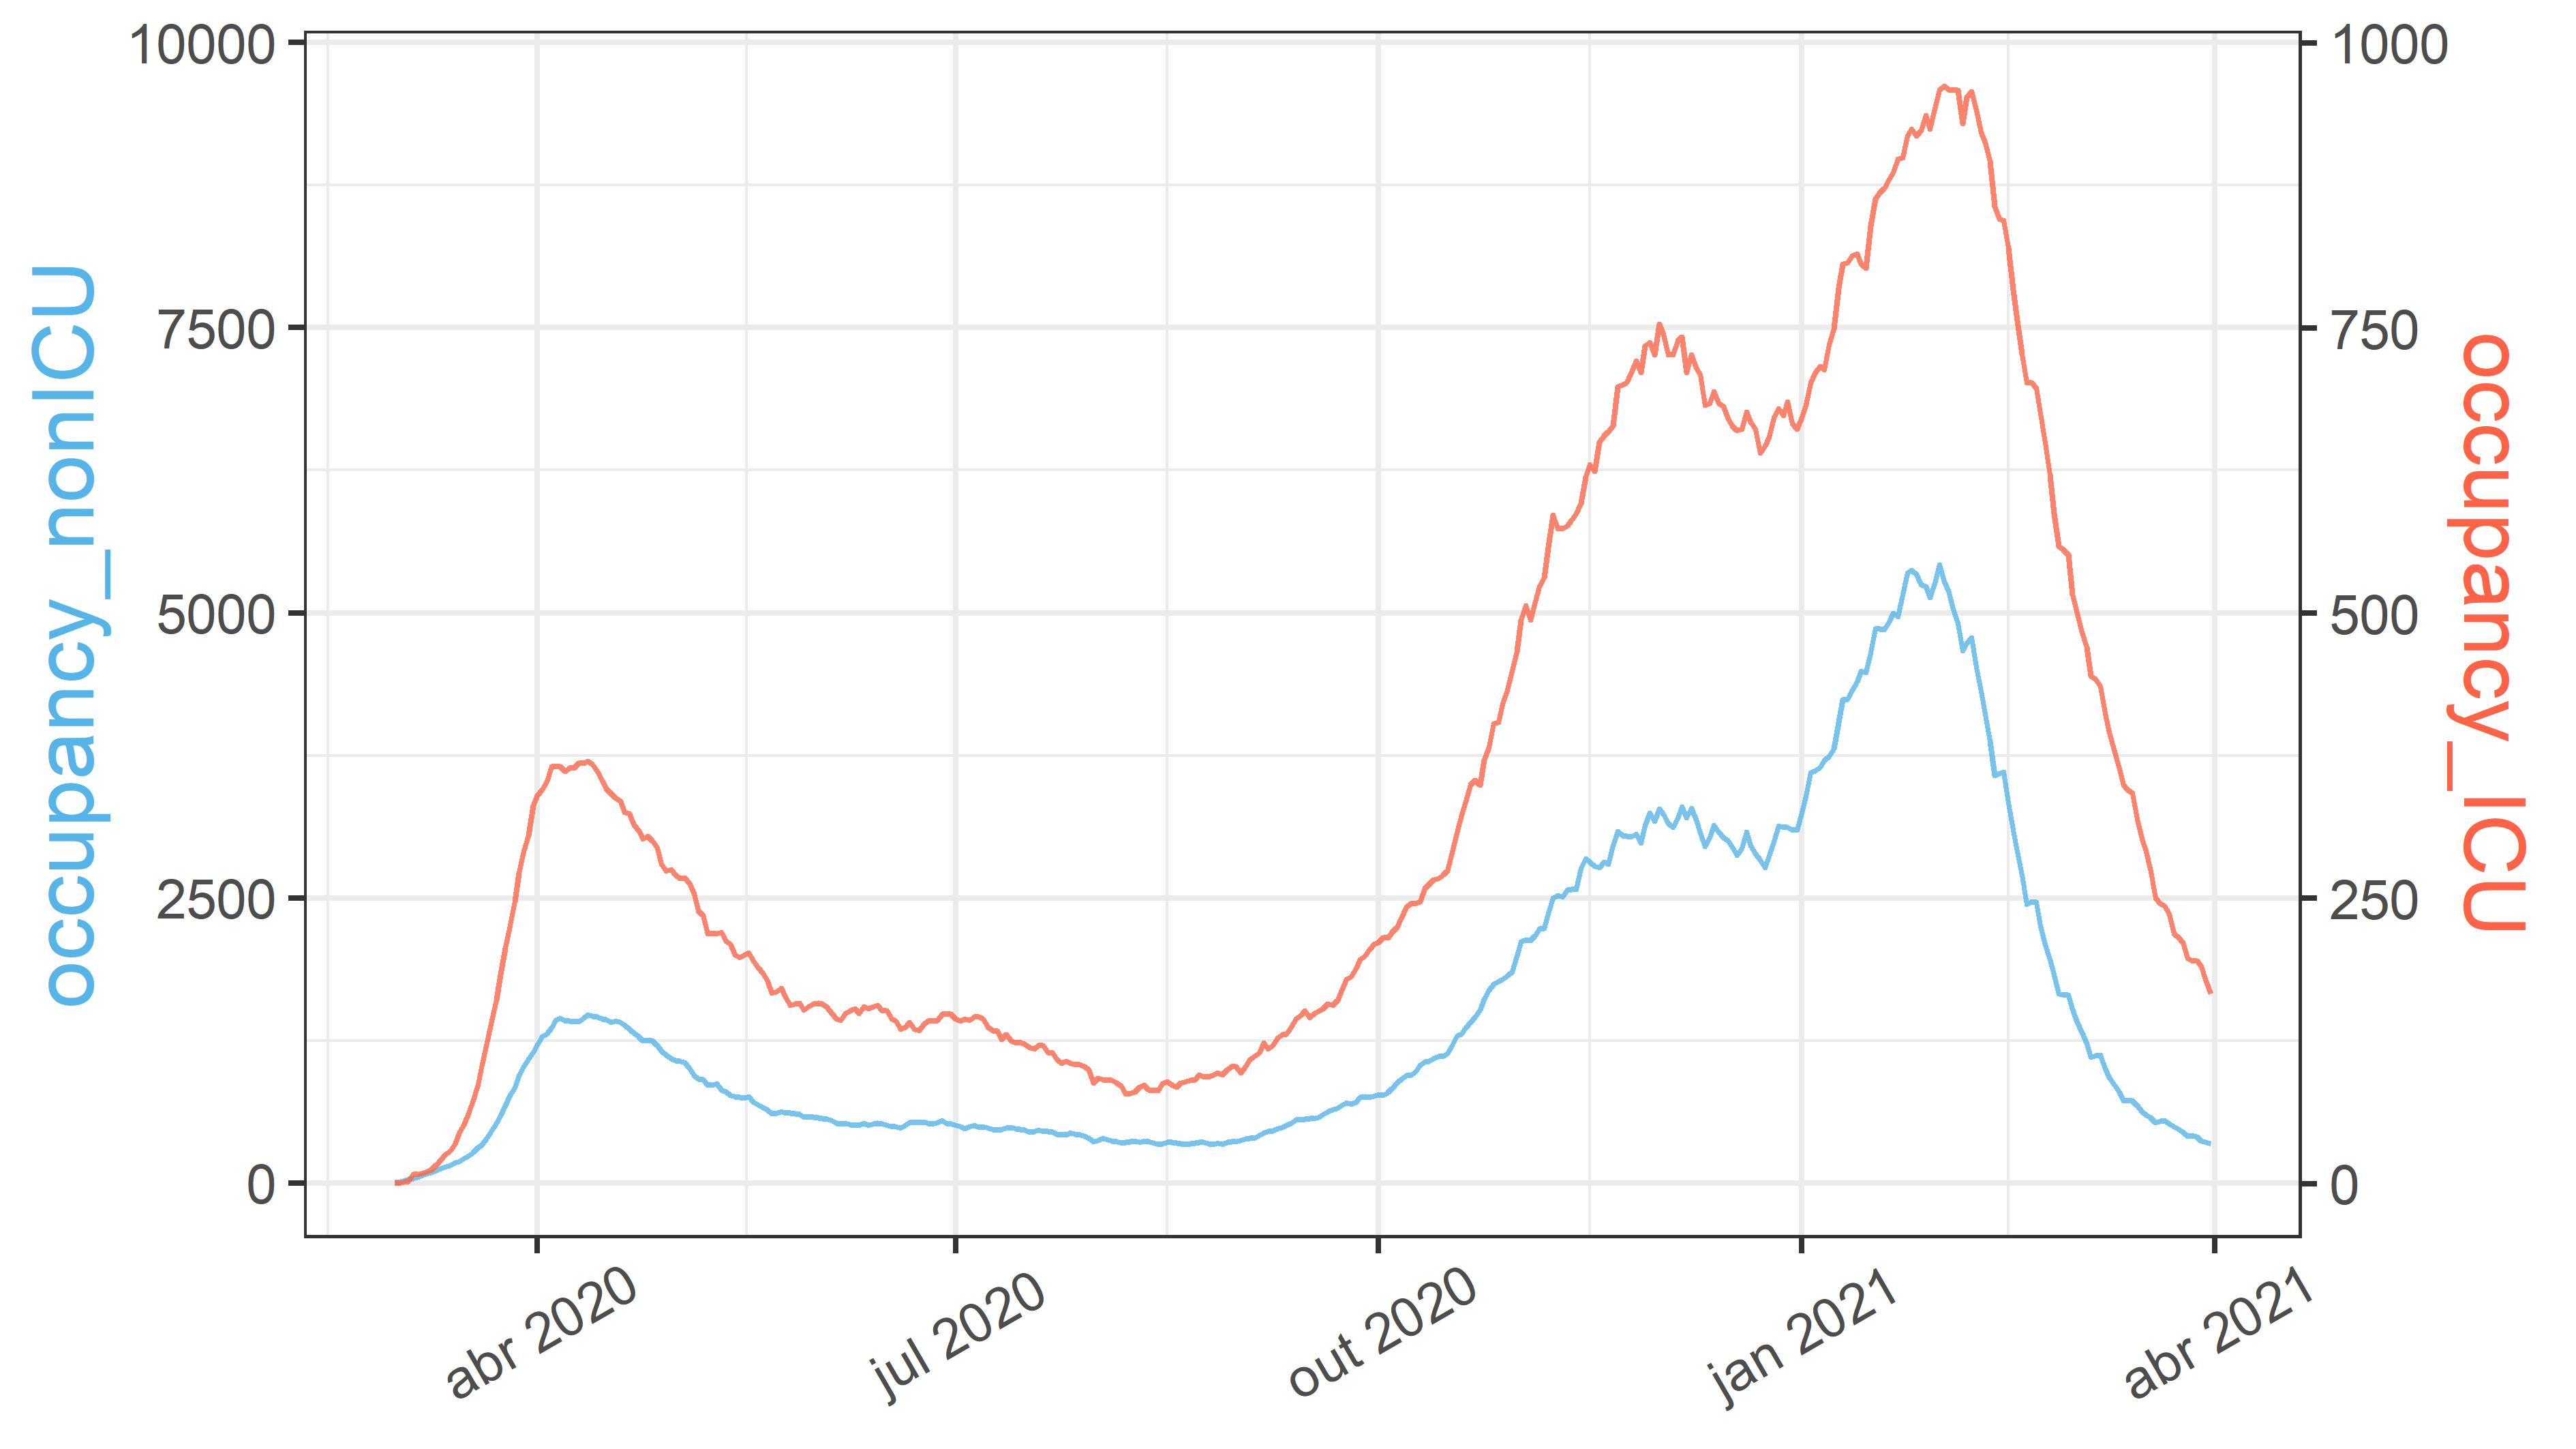
\includegraphics[width=\textwidth]{Imagens/byDayPlot_inHosp.jpeg}
\end{subfigure}
\begin{subfigure}{0.3\textwidth}
\caption*{Género}
\vspace{-0.4cm}
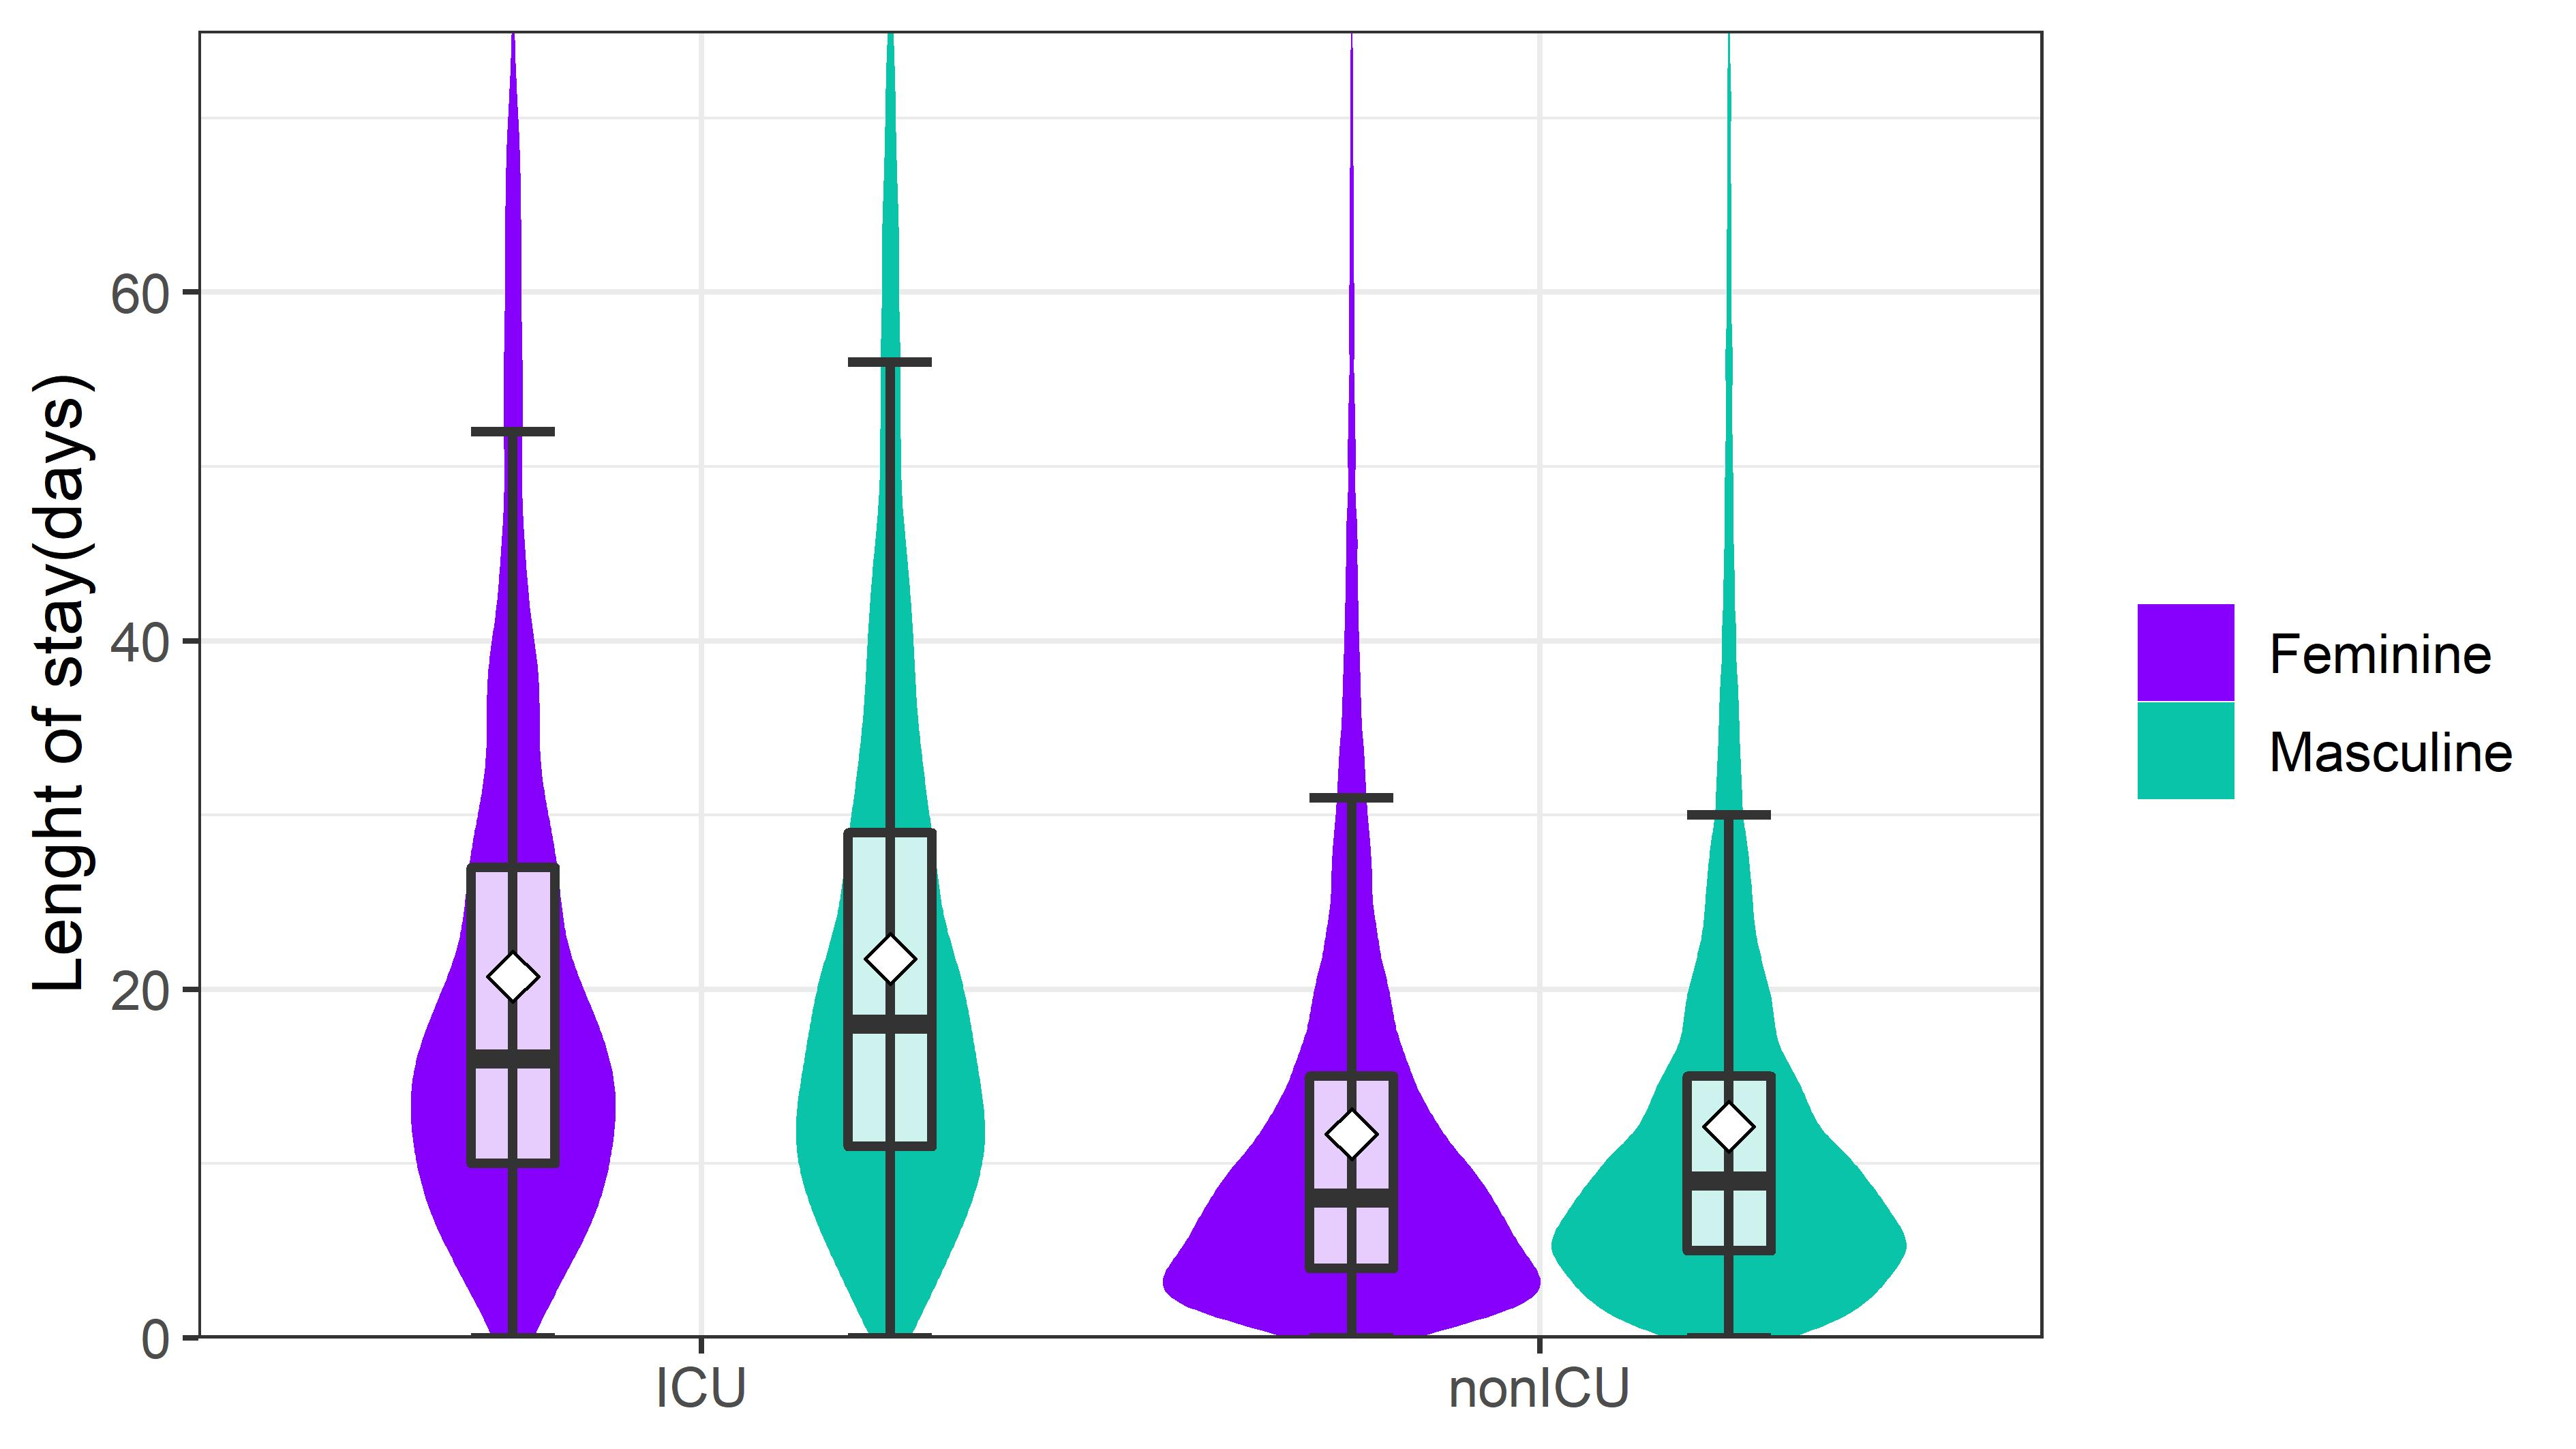
\includegraphics[width=\textwidth]{Imagens/violinBox_Gender.jpeg}
\end{subfigure}
\begin{subfigure}{0.3\textwidth}
\caption*{Tempo}
\vspace{-0.4cm}
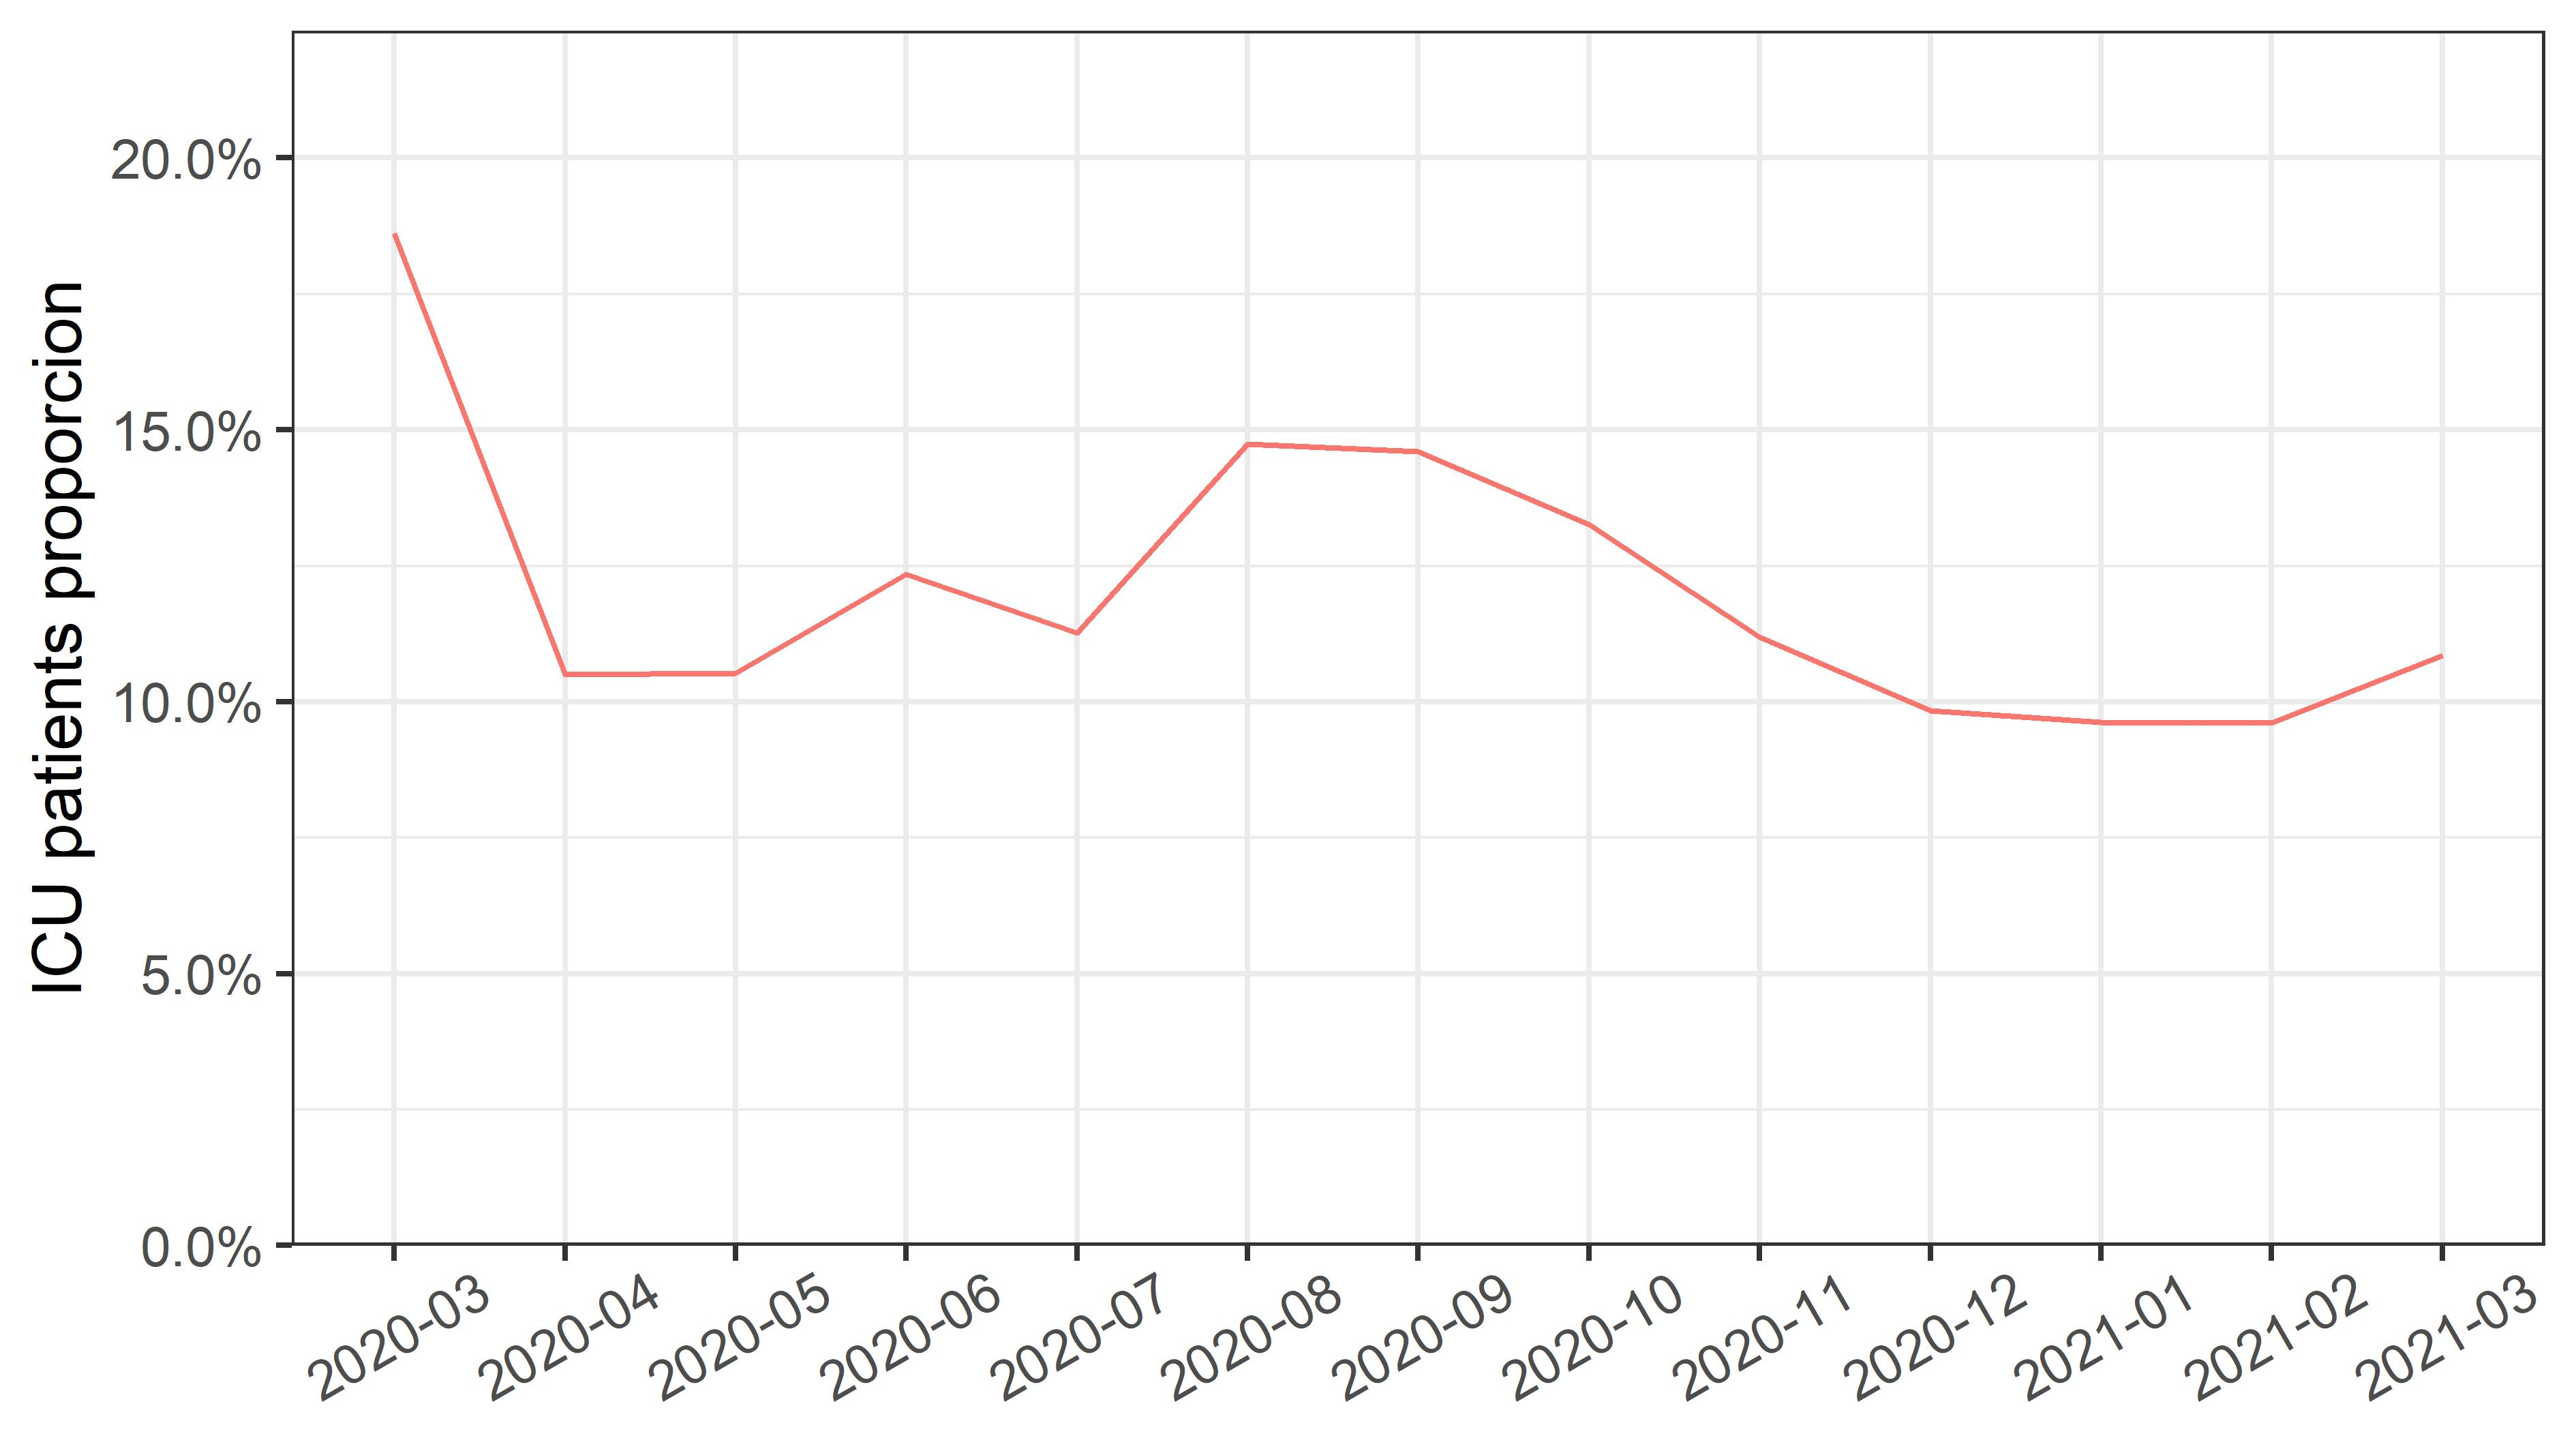
\includegraphics[width=\textwidth]{Imagens/PopVarPlot_PropICU.jpeg}
\end{subfigure}
\begin{subfigure}{0.3\textwidth}
\caption*{Grupo etário}
\vspace{-0.4cm}
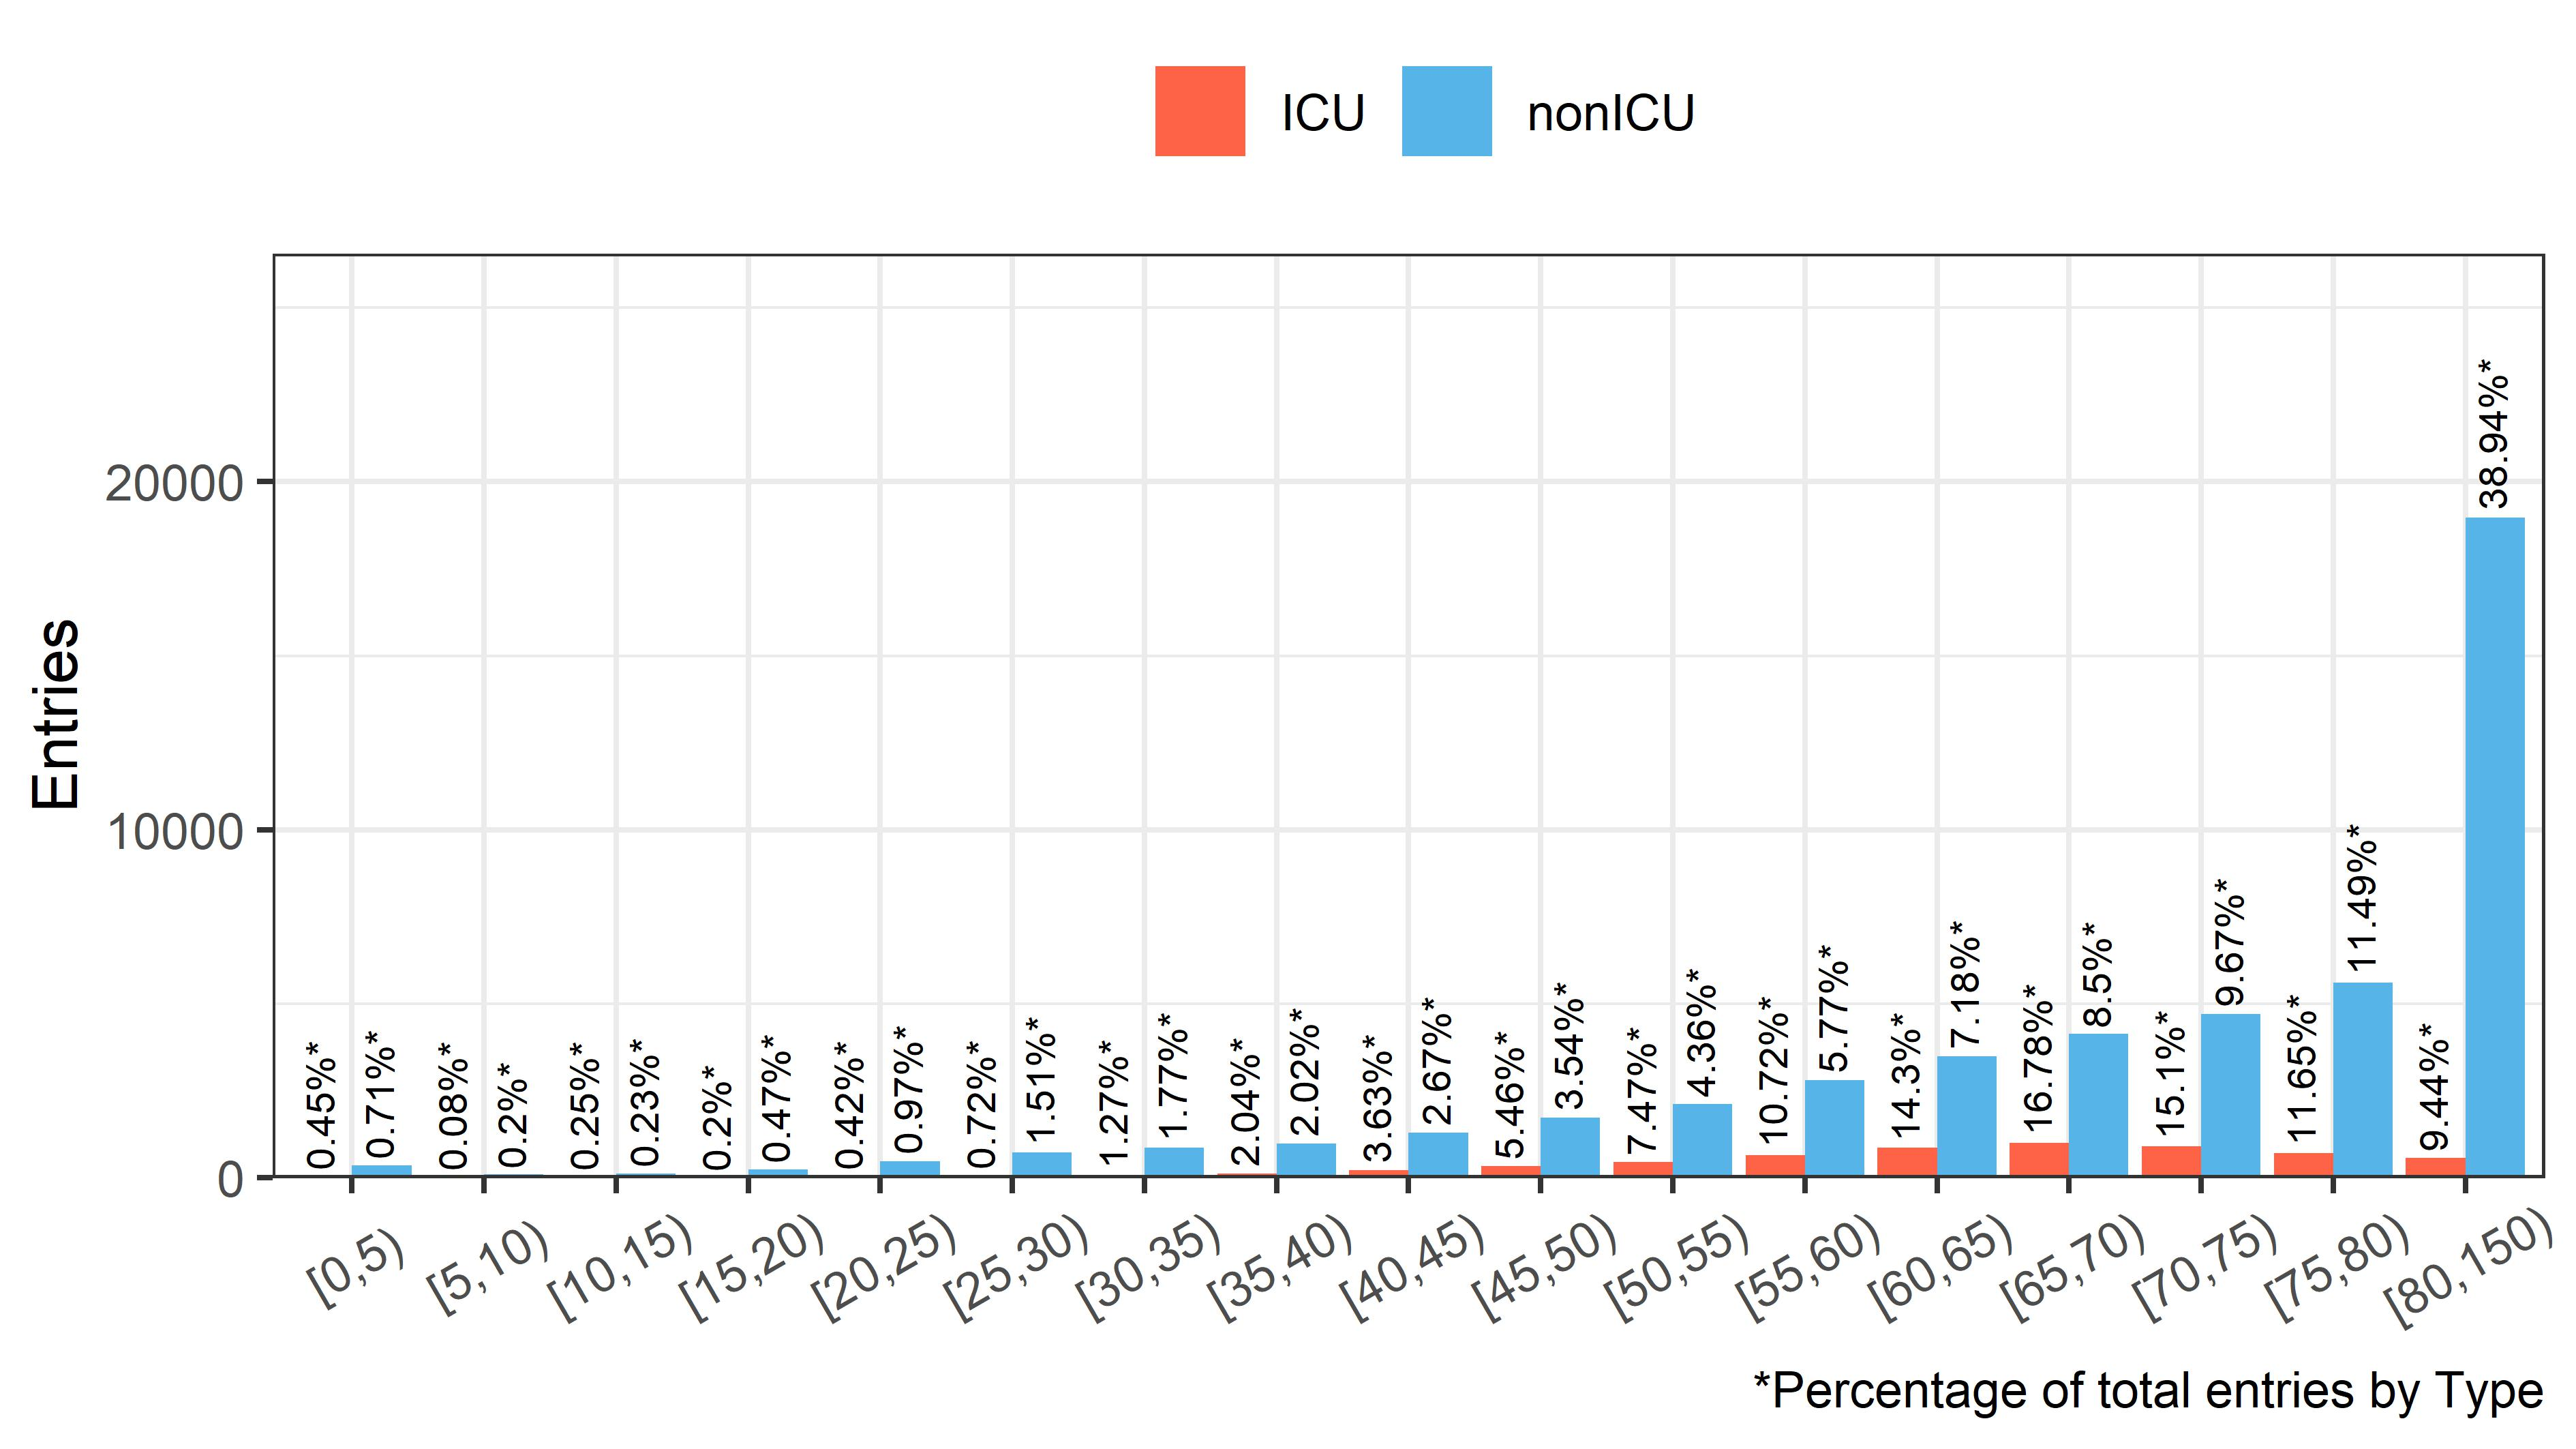
\includegraphics[width=\textwidth]{Imagens/histPlot_Group_Type.jpeg}
\end{subfigure}
\begin{subfigure}{0.3\textwidth}
\caption*{Região}
\vspace{-0.4cm}
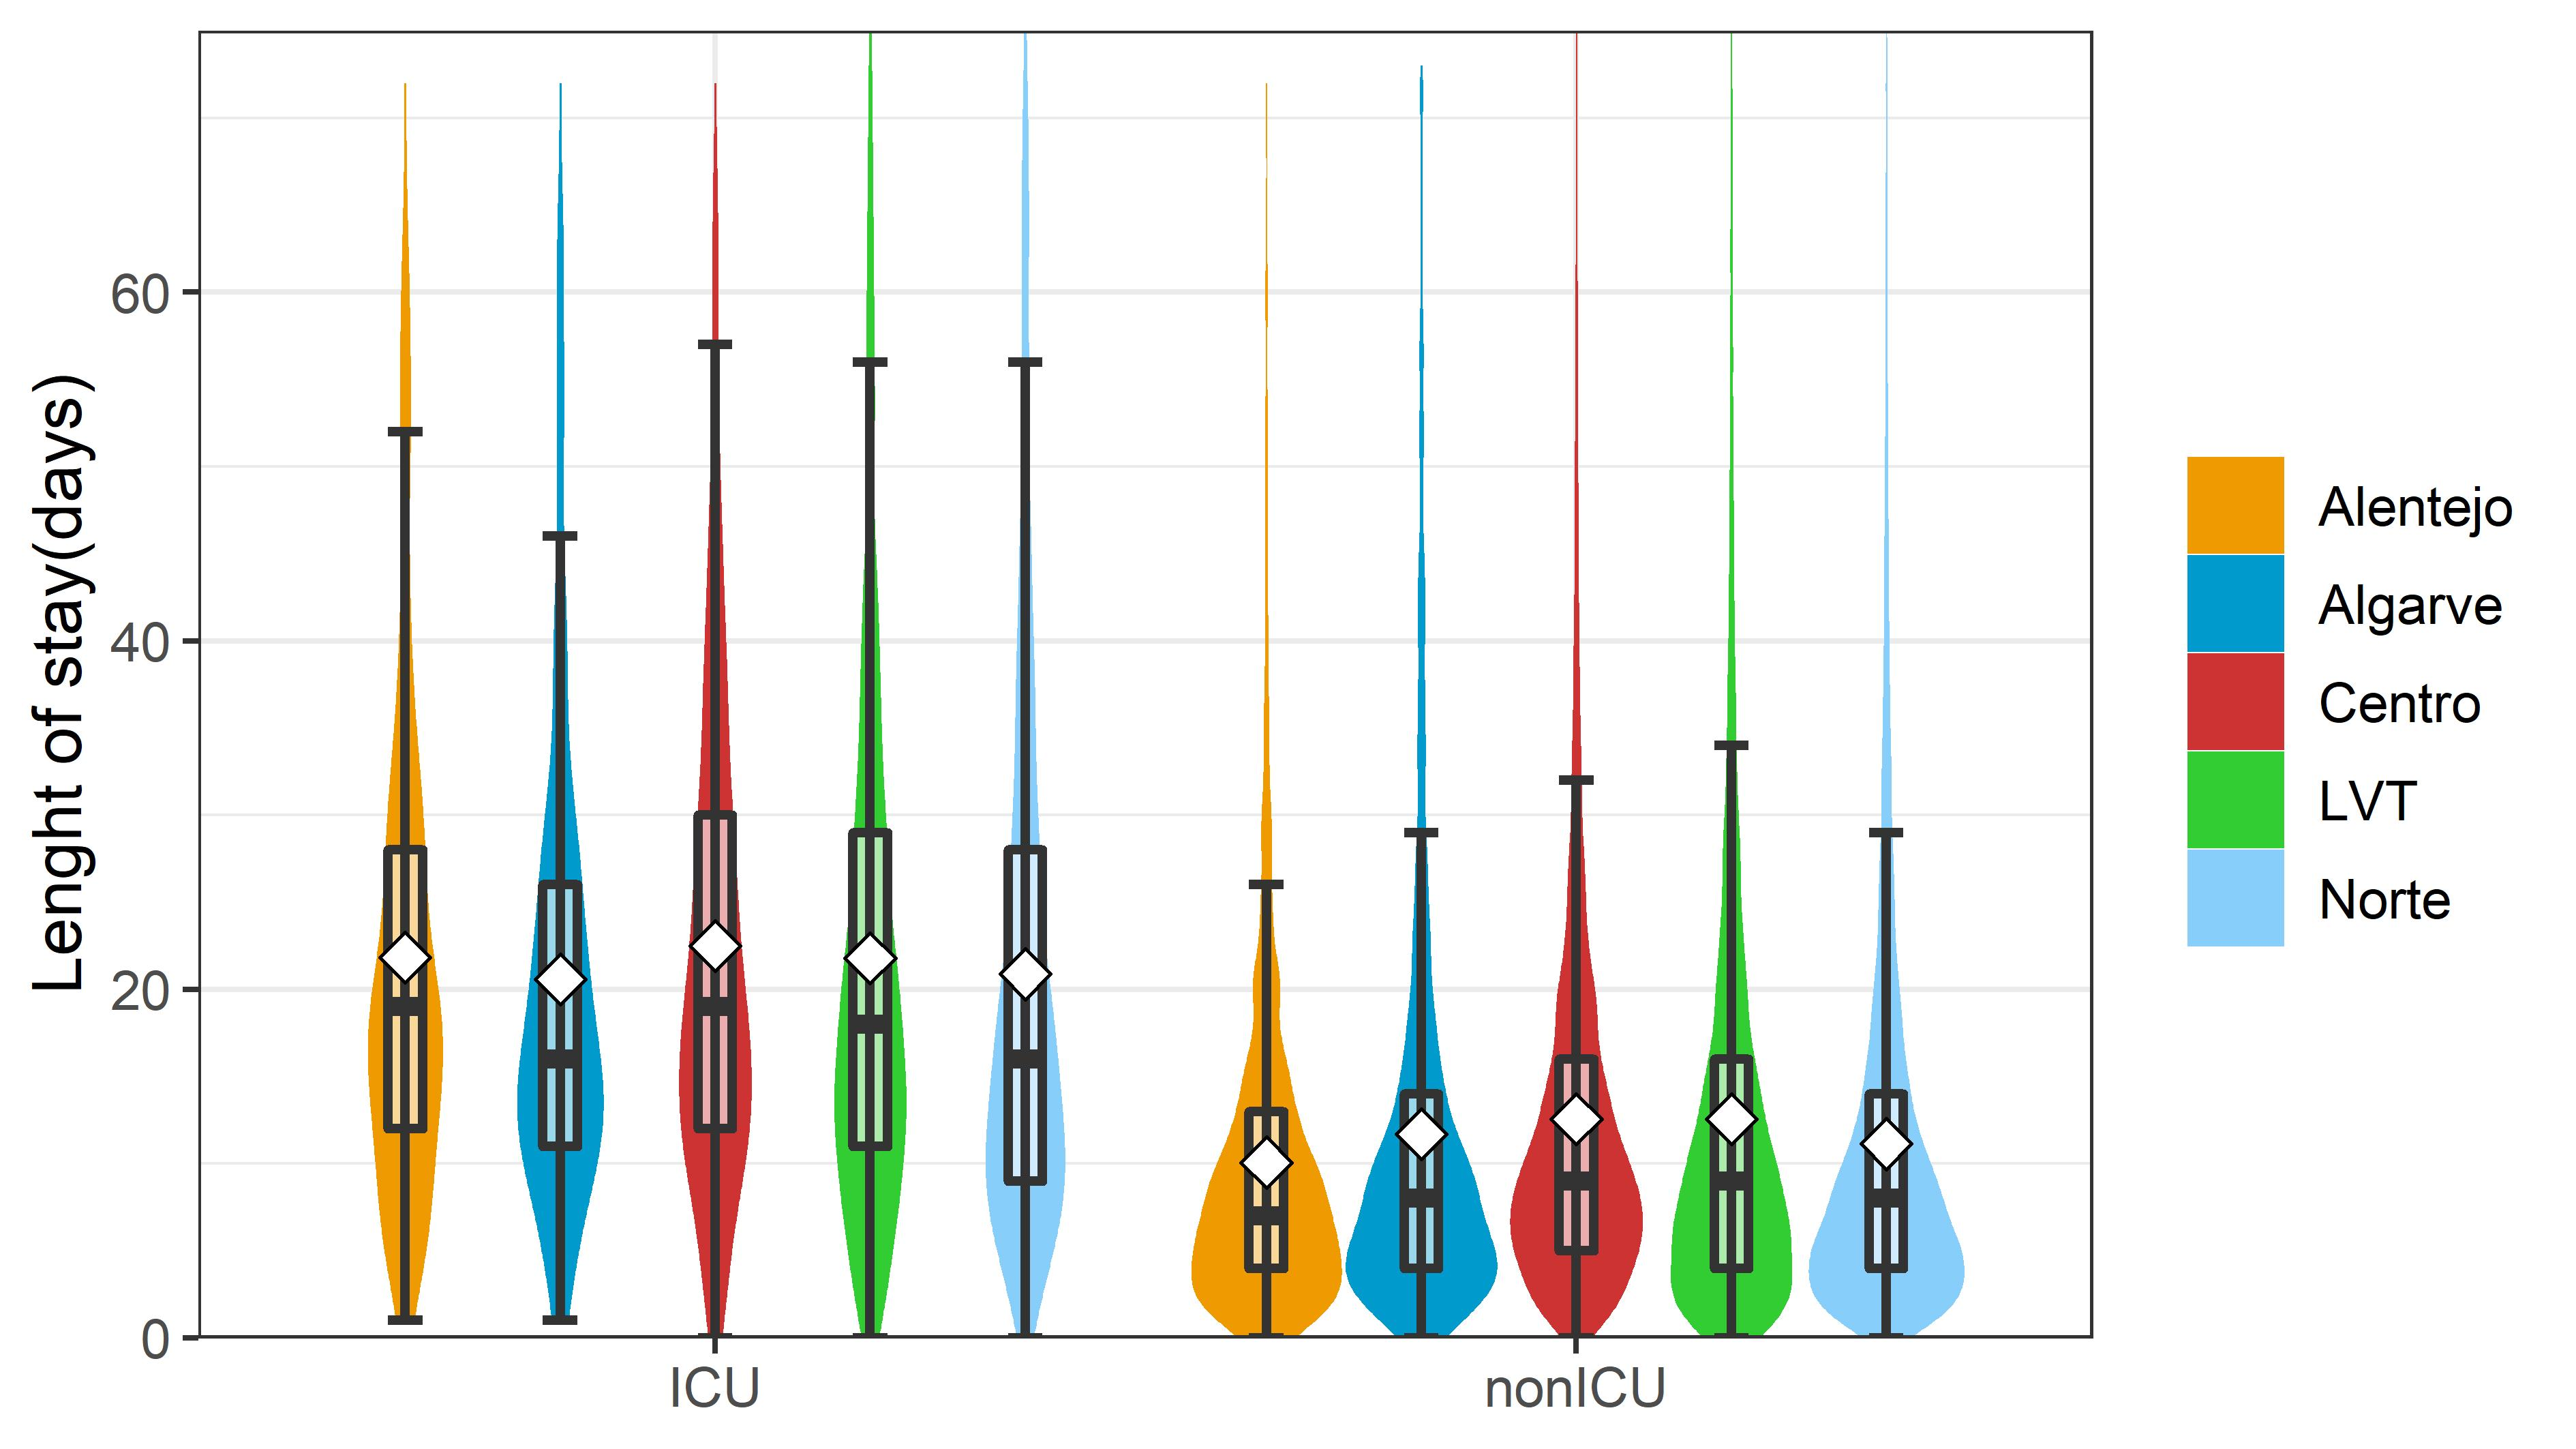
\includegraphics[width=\textwidth]{Imagens/violinBox_Region.jpeg}
\end{subfigure}
\begin{subfigure}{0.3\textwidth}
\caption*{Resultado da hospitalização}
\vspace{-0.4cm}
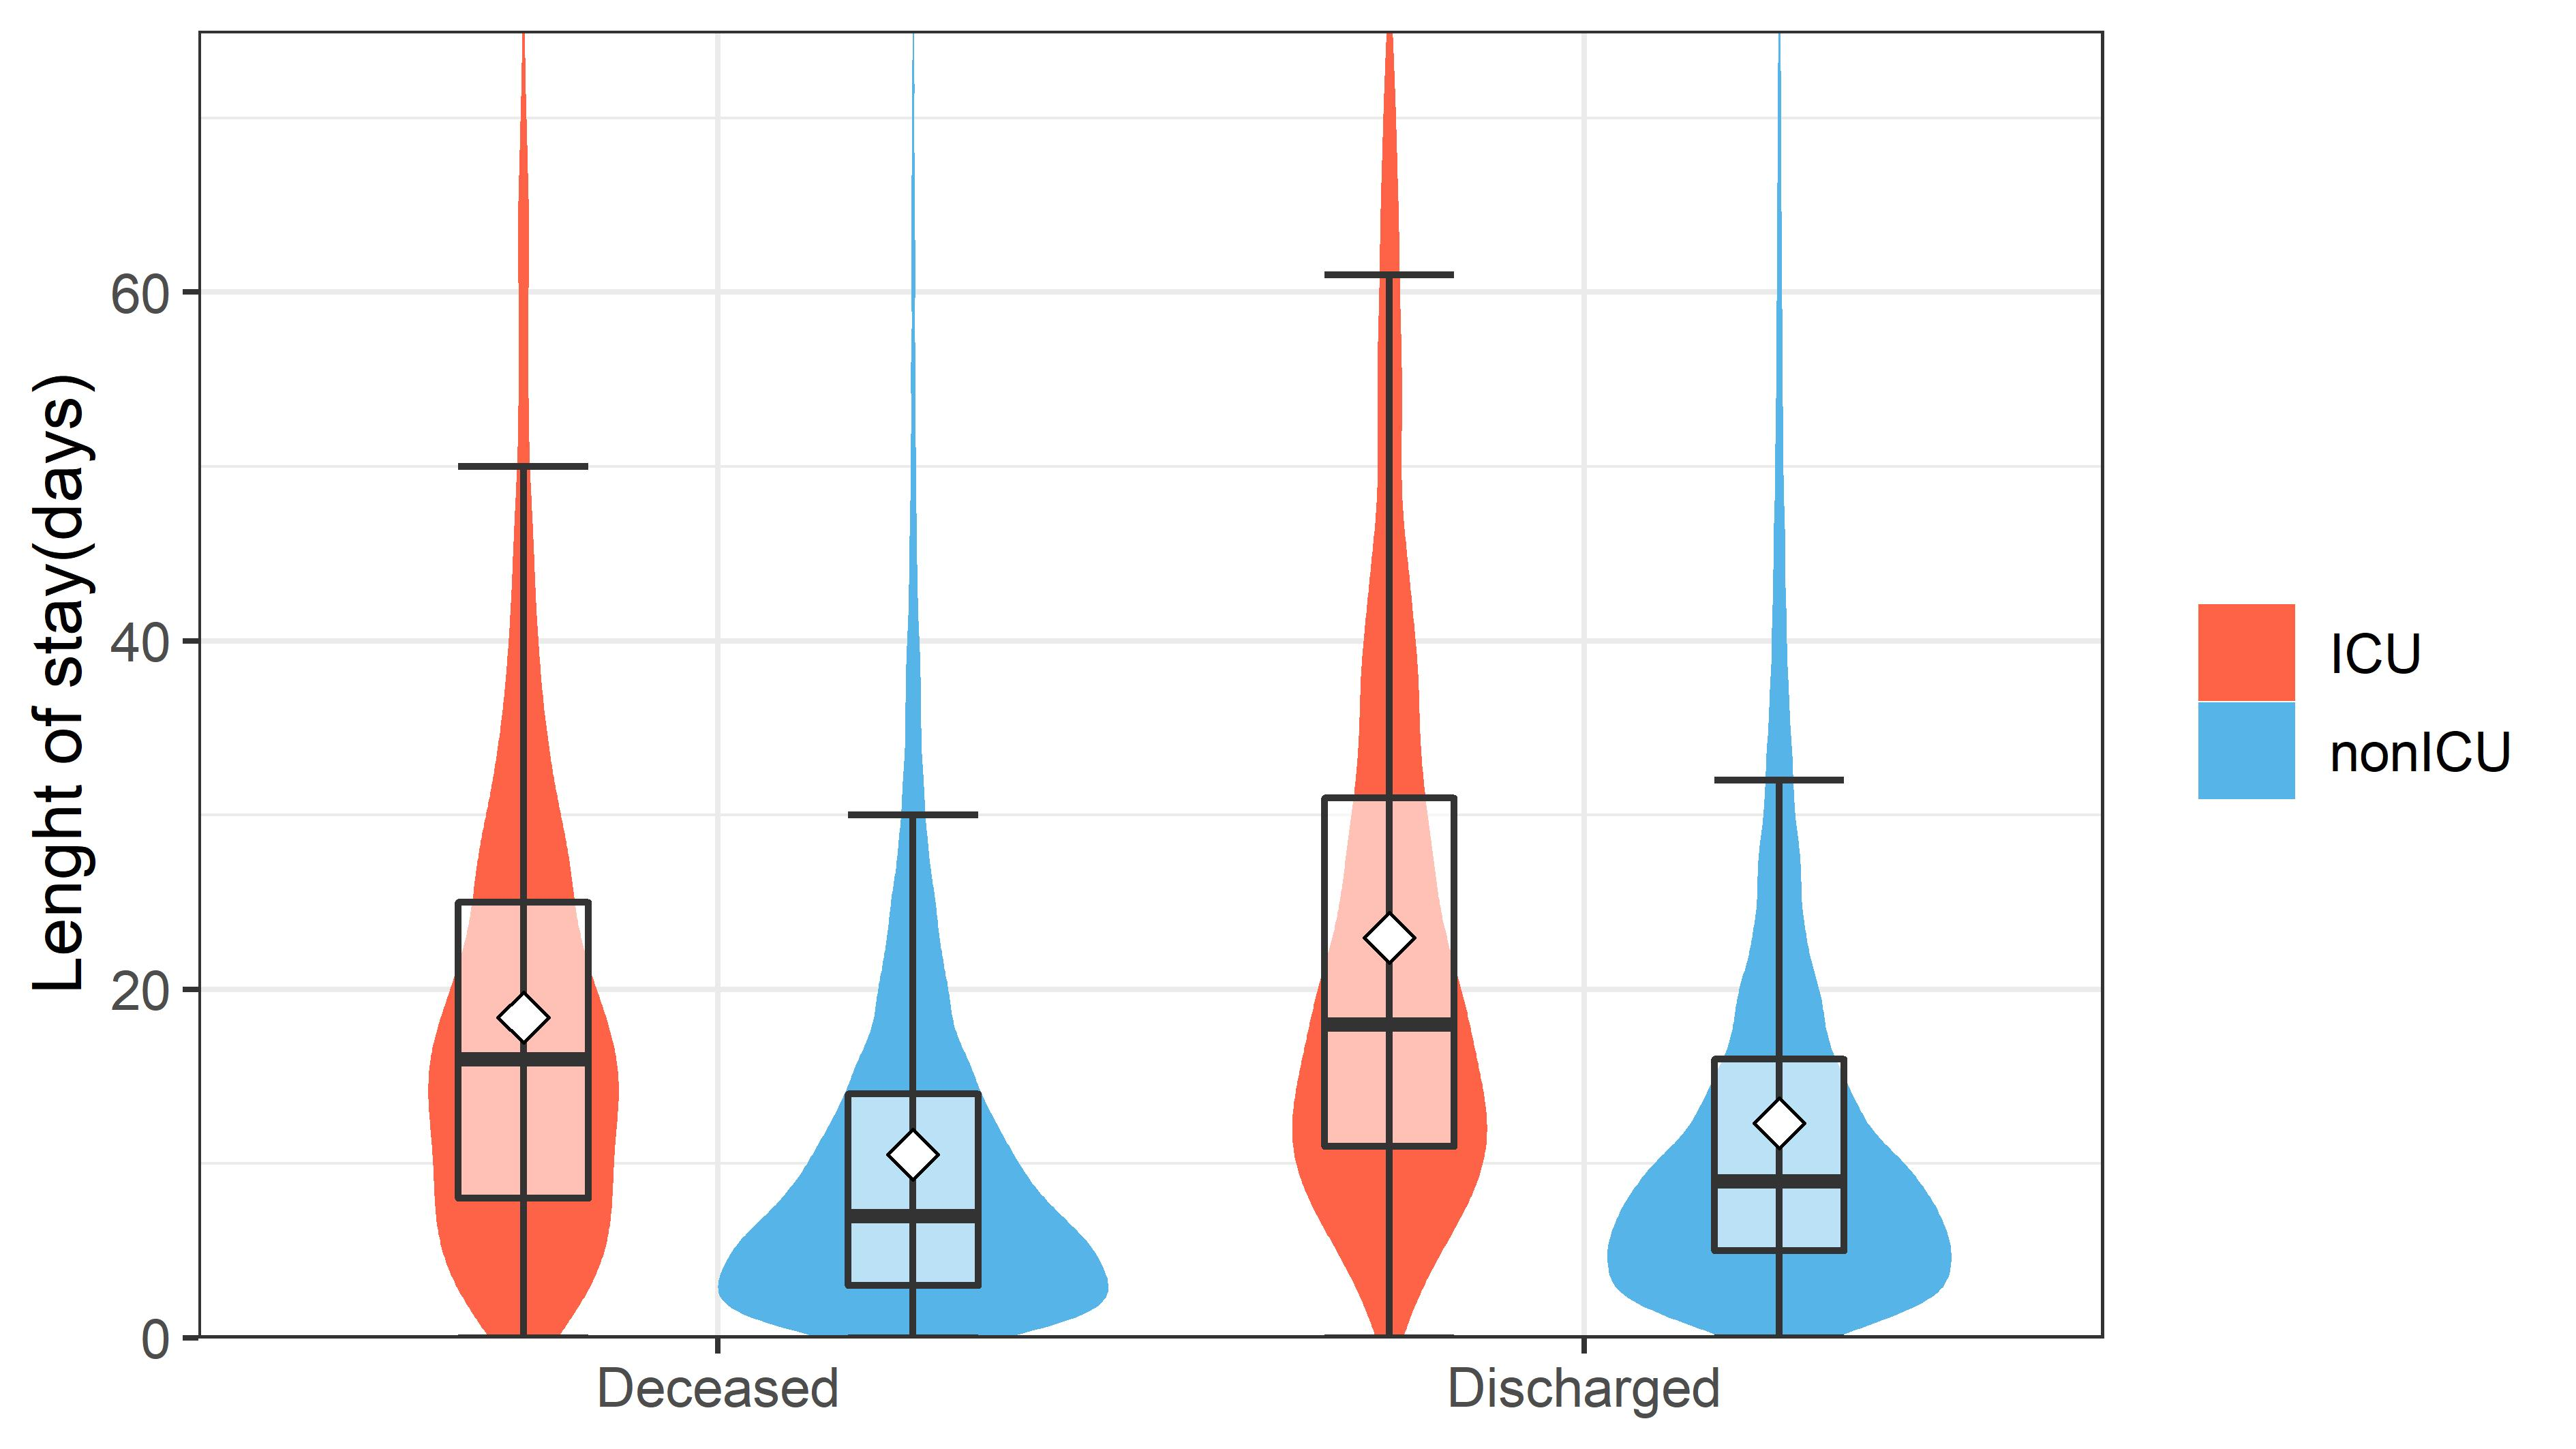
\includegraphics[width=\textwidth]{Imagens/violinBox_Outcome.jpeg}
\end{subfigure}
\end{figure}

\end{frame}

%% Resultados
\begin{frame}{Resultados}
\vspace{0.4cm}
\textbf{Objetivo:} Identificar variáveis e relações de interesse para a questão em estudo.

\begin{columns}
	\begin{column}[T]{0.65\textwidth}
	\scalebox{0.45}{$
		\begin{aligned}
            		\text{Proporção de pacientes UCI} &= \frac{\text{entradas UCI}}{\text{Total entradas}} \times 100\% = 10.92\% \\
            		\\
		            \text{Mortalidade de pacientes ICU} &= \frac{\text{fatalidades não-UCI}}{\text{entradas não-UCI}} \times 100\% = 22.60\% \\
		            \\
		            \text{Mortalidade de pacientes não-UCI} &= \frac{\text{fatalidades UCI}}{\text{entradas UCI}} \times 100\% = 32.84\%
        		\end{aligned}
	$}
	\vspace{0.2cm}
	\begin{figure}
		\caption*{\small Parâmetros de interesse, em relação a várias variáveis}
		\vspace{-0.2cm}
		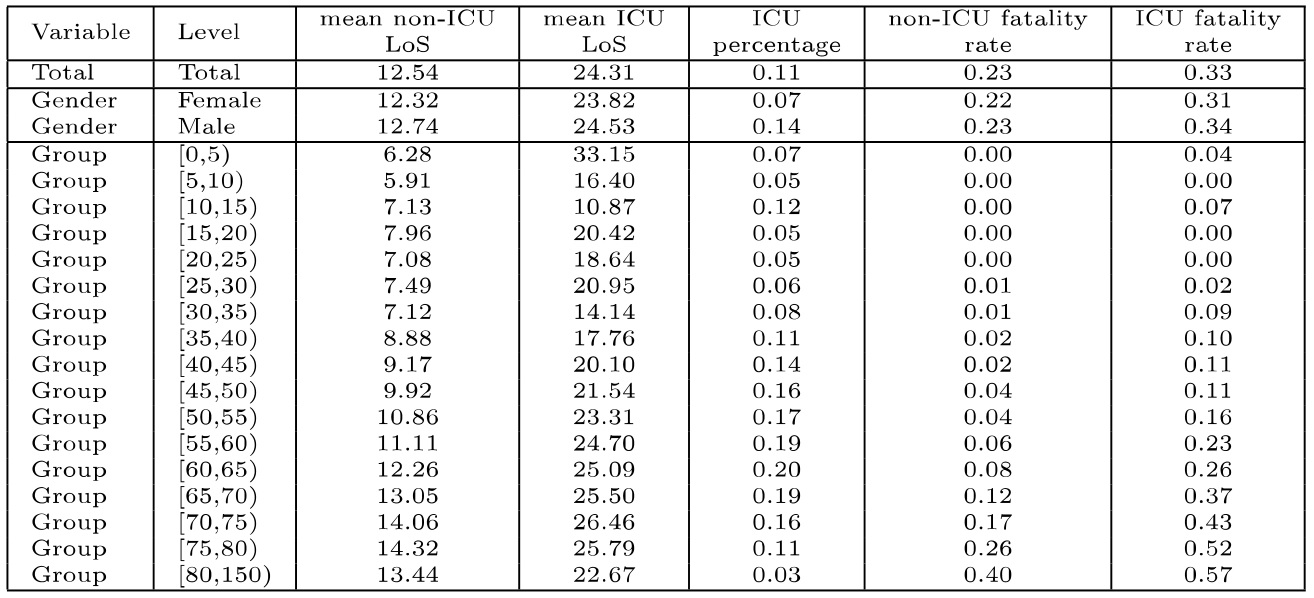
\includegraphics[width=0.8\textwidth]{Imagens/Tabela_params.jpg}
	\end{figure}
	\end{column}
	
	\begin{column}[T]{0.35\textwidth}
	\begin{figure}
		\caption*{\small Ajuste a distribuições estatísticas}
		\vspace{-0.2cm}
		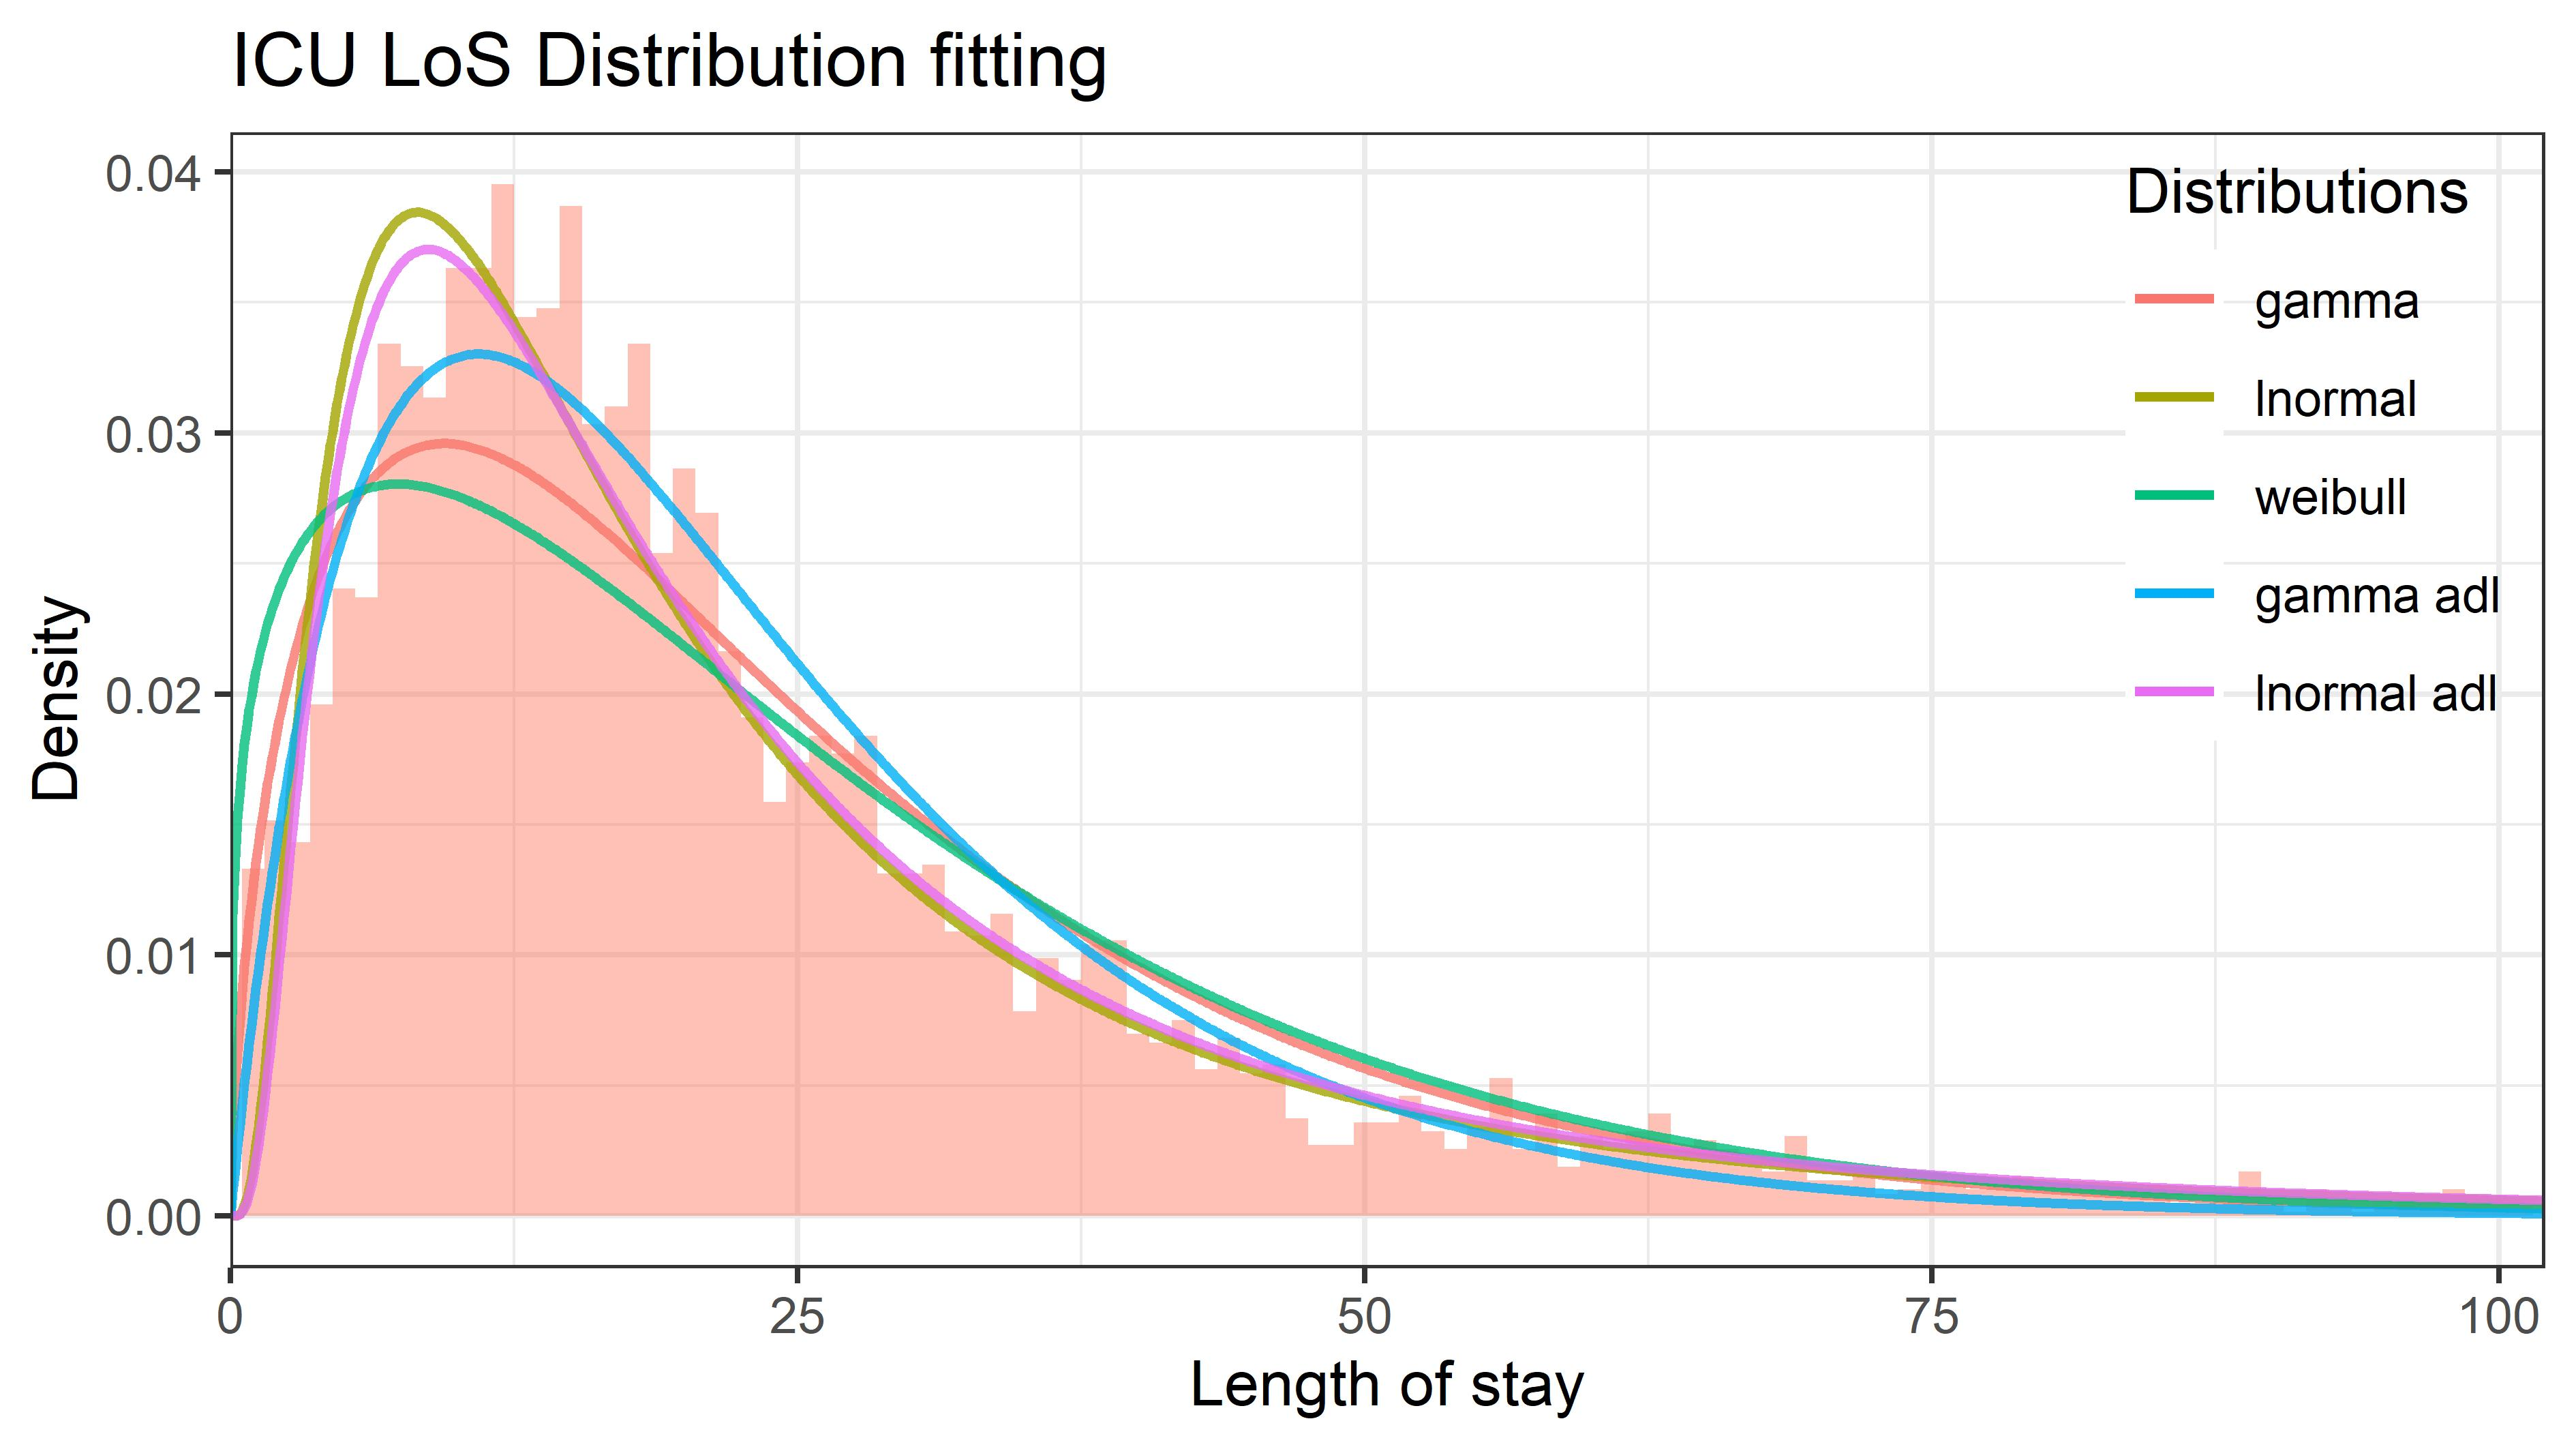
\includegraphics[width=\textwidth]{Imagens/distFit_ICU.jpeg}
	\end{figure}
	\end{column}
\end{columns}
\end{frame}

%% Resultados 2
\begin{frame}{Resultados}
%\begin{columns}
%	\begin{column}[T]{0.65\textwidth}
		\textbf{Permitindo tirar as seguintes conclusões de maior interesse:}
		\vspace{0.5cm}
		\begin{itemize}
			\item Pacientes UCI passam mais tempo em hospital, independentemente do resultado
			\item Idade condiciona taxa de hospitalização, tempo de permanência, entre outros
			\item Homens são mais hospitalizados em UCI, mas tem igual tempo de permanecia e taxa de mortalidade
			\item Percentagem pacientes UCI e taxa de mortalidade variaram ao longo do tempo
		\end{itemize}
%	\end{column}
	
%	\begin{column}[T]{0.35\textwidth}
	
%	\end{column}
%\end{columns}
\end{frame}

\begin{frame}{Demonstração Prática}

\alert{\Large Convido todos os presentes a acompanharem a demonstração nos seus computadores.}
\vspace{0.4cm}
\centering

A demonstração encontra-se disponível em :
\vspace{0.2cm}
\scriptsize{
\url{https://github.com/Pereirajpf/XXX.git}
}

\vspace{0.4cm}

, bem como os ficheiros desta apresentação em:
\vspace{0.2cm}
\tiny{
\url{https://github.com/Pereirajpf/Thesis_Presentation_JPereira.git}
}


\includegraphics[width=0.2\textwidth]{Imagens/qrcode_apresentação.png}
\end{frame}

%%
\end{document}

